\documentclass[article]{jss}

%% -- LaTeX packages and custom commands ---------------------------------------

%% recommended packages
\usepackage{orcidlink,thumbpdf,lmodern}
\usepackage{amsmath,amssymb,bm}
\usepackage{placeins}

%% custom math shortcuts kept minimal — JSS prefers light macro use
\newcommand{\fct}[1]{\code{#1()}}


%% -- Article metainformation (author, title, ...) -----------------------------

\author{Artur Sepp\\LGT Bank
\And Mika A. Kastenholz\\LGT Bank}
\Plainauthor{Artur Sepp, Mika A. Kastenholz}

\title{\pkg{factorlasso}: Sparse Multi-Output Regression with
Cluster-Grouped Sign Constraints in \proglang{Python}}
\Plaintitle{factorlasso: Sparse Multi-Output Regression with
Cluster-Grouped Sign Constraints in Python}
\Shorttitle{\pkg{factorlasso}: Sparse Multi-Output Regression in \proglang{Python}}

\Abstract{
Many regression problems require a coefficient matrix that maps a set of
predictors to several related responses, where the responses fall into
groups that share the sign of their loadings, the sample is short, and the
predictors are correlated. Multi-asset factor modelling in finance is a
leading instance. The \pkg{factorlasso} \proglang{Python} package fits such
models through a \pkg{scikit-learn}-style \code{fit}/\code{predict}
interface built on \pkg{CVXPY}. It implements a family of sparse estimators,
the LASSO, the group LASSO, the sparse group LASSO, adaptive weighting,
univariate-guided regression, and the cooperative LASSO, as configurations
of one objective, and adds three capabilities that, to our knowledge, no
surveyed package combines: cluster structure obtained from the response
correlation matrix, cell-level sign constraints derived from a
cluster-pooled univariate slope and gated by a noise-floor $t$~statistic,
and prior-centred shrinkage toward a non-zero baseline. The gated
cluster-pooled sign mechanism and its consistency theory are developed in a
companion methodology paper. On a data-generating process calibrated to a
publicly reproducible $102$-asset multi-asset exchange-traded-fund universe
with known true loadings, three competing \proglang{Python} packages match
\pkg{factorlasso} on coefficient error and out-of-sample fit, yet only its
sign- and prior-constrained configuration keeps the collinear credit
factor on a correctly signed, non-zero loading, where zero-centred
shrinkage collapses it into equity. The package ships a
reproducible simulation and application harness and is available from the
Python Package Index under the GNU General Public License.
}

\Keywords{sparse regression, group LASSO, sign constraints,
hierarchical clustering, adaptive LASSO, factor model,
multi-response regression, \proglang{Python}, \pkg{CVXPY}}
\Plainkeywords{sparse regression, group LASSO, sign constraints,
hierarchical clustering, adaptive LASSO, factor model,
multi-response regression, Python, CVXPY}

\Address{
Artur Sepp\\
Global Head of Quantitative Analytics\\
LGT Bank\\
E-mail: \email{artur.sepp@lgt.com}\\
URL: \url{https://github.com/ArturSepp/factorlasso}\\[2mm]
Mika A. Kastenholz\\
Global Head of Investment Solutions\\
LGT Bank\\
E-mail: \email{mika.kastenholz@lgt.com}
}


\begin{document}


%% -- Introduction -------------------------------------------------------------

\section[Introduction]{Introduction} \label{sec:intro}

Multi-output sparse regression estimates a coefficient matrix
$\bm{\beta} \in \mathbb{R}^{N \times M}$ that maps $M$ predictors to $N$
related responses. In many applications the responses fall into groups
whose members share the sign of their loading on a common predictor, the
sample length $T$ is short relative to the number of parameters, and the
predictors are correlated. An estimator that exploits the shared group
structure and the known signs can outperform one that treats each response
independently. A leading instance is the multi-asset factor model in
quantitative finance, which underpins the commercial risk systems in
industry use, among others MSCI Barra, Axioma, and Bloomberg's
multi-asset-class models. These systems decompose asset returns into a few
common factors and an idiosyncratic residual
\citep{Rosenberg+McKibben:1973, Connor:1995}. There the responses are the
$N$ asset returns, the predictors are $M$ tradable factors, and the sample
is $T$ periods, and the estimation regime is adverse on four counts. First,
the sample is short by statistical standards, because most core cross-asset
indices and funds launched in the late 2000s and 2010s, giving 5 to 25 years
of data. Second, the factors are often strongly correlated, so the design
carries severe multicollinearity. Third, the cross-section is moderate
($N \in [50, 200]$ at the multi-asset-class level). Fourth, the true
coefficient matrix exhibits a cluster structure that the practitioner does
not know a priori, and traditional provider-based asset classifications are
a weak proxy for the interdependence of assets. Assets in the same economic
group, such as regional equity, investment-grade credit, or hedge funds,
typically share signs on the dominant factors.


Sparse regression has a long history of methodology and software for
each component of this problem in isolation. The LASSO of
\cite{Tibshirani:1996} produces a sparse coefficient vector via $\ell_1$
penalisation, the group LASSO of \cite{Yuan+Lin:2006} produces sparse
group selection via the $\ell_2$-of-each-group penalty, the sparse group
LASSO of \cite{Simon+Friedman+Hastie+Tibshirani:2013} mixes the two,
and the adaptive LASSO of \cite{Zou:2006} and its group extension by
\cite{Wang+Leng:2008} reweight the penalty by univariate evidence to
recover the oracle property. The univariate-guided LASSO of
\cite{Chatterjee+Hastie+Tibshirani:2025} uses univariate slope signs
as hard constraints on the multivariate problem. The biobank-scale
extension of \cite{Richland+Kiiskinen+Wang+Lu+Narasimhan+Hastie+Rivas+Tibshirani:2025}
combines univariate sign constraints with adaptive reweighting on
genome-wide data with millions of candidate predictors. The
high-dimensional sparse-recovery view of penalised regression goes
back to \cite{Vattikuti+Lee+Chang+Hsu+Chow:2014}, who apply
compressed sensing to genome-wide association data and document a
sharp sample-size threshold for support recovery. Hierarchical clustering of the response
correlation matrix, as in \cite{Bondell+Reich:2008} and extensively
applied in financial portfolio construction by
\cite{LopezdePrado:2016}, recovers data-driven groups suitable for use
as the group structure in group LASSO.

The combination of sparsity, sign constraints, and cluster consistency,
however, is not available as a single coherent software artifact. In
the \proglang{Python} ecosystem, \pkg{scikit-learn}'s \code{Lasso}
class \citep{Pedregosa+etal:2011} handles the basic single-response
LASSO with no group structure and no multi-response capability. The
\pkg{group-lasso}, \pkg{asgl}
\citep{Mendez-Civieta+Aguilera-Morillo+Lillo:2021}, and \pkg{celer}
\citep{Massias+Gramfort+Salmon:2018} packages handle group
LASSO with externally specified groups but do not perform cluster
discovery and do not implement sign constraints at the cell level. The
\pkg{adelie} package \citep{Yang+Hastie:2024} provides a fast
multi-task group LASSO solver but again requires the group structure as
an input. Beyond \proglang{Python}, the \proglang{R} packages
\pkg{gglasso} \citep{Yang+Zou:2015}, \pkg{sparsegl}
\citep{Liang+Cohen+SolonHeinsfeld+Pestilli+McDonald:2024}, and
\pkg{oem} cover overlapping subsets of this
surface. None of these packages combines cluster discovery,
cluster-pooled sign derivation with a noise-floor gate, adaptive
penalty reweighting routed through both the $\ell_1$ and group $\ell_2$ paths, and
prior-centred regularisation toward a non-zero baseline. Financial-panel
estimation requires all four together.

The \pkg{factorlasso} package, presented in this paper, supplies that
combination. Specifically, \pkg{factorlasso} implements:

\begin{enumerate}
\item Multi-response sparse regression on the loading matrix
$\beta \in \mathbb{R}^{N \times M}$ in a single convex programme,
with the cross-asset information entering through a
\emph{precomputed} cluster-pooled sign matrix and adaptive
penalty weights rather than through a cross-asset group norm.
Hierarchical clustering group LASSO (HCGL) discovers the cluster
structure by Ward linkage on the response correlation matrix and
uses it to pool the sign derivation and the adaptive weights. Given
the sign matrix and weights, the programme is block-separable across
assets and reduces to $N$ per-asset second-order cone problems
solved as one object.
\item Cluster-pooled univariate sign derivation: the univariate slope
computed against the cluster-mean response and broadcast to every
cluster member as a hard sign constraint, gated by a noise-floor
$t$~statistic that pins weak-evidence cells to zero. A closed-form
residual sum-of-squares (SSR) identity vectorises the gate across
factors \citep{Sepp+Kastenholz:2026sign}.
\item Adaptive penalty reweighting following \cite{Zou:2006} and
\cite{Wang+Leng:2008}, routed through both the $\ell_1$ and group $\ell_2$ paths
and driven by the same pooled slope that produces the sign matrix.
\item Prior-centred regularisation, in which the penalty pulls toward
an economically motivated $\beta^{0} \neq 0$ rather than toward zero.
\item Consistent factor covariance assembly, in which the same
$\beta$ matrix used in the conditional mean is reused in the implied
covariance, producing alpha-beta consistency by construction (\cite{Sepp+Hansen+Kastenholz:2026MATF}).
\end{enumerate}

The cluster layer that drives the sign-derivation pooling and the
cluster-size penalty weights differentiates the package from a configurable
sparse-group LASSO solver such as \pkg{asgl} or \pkg{sparsegl}. The clusters
are not external inputs but discovered from the data, and the same partition
feeds the sign-derivation pooling, the cluster-size penalty weights, and the
row-aggregation for adaptive reweighting. The gated cluster-pooled
sign-derivation mechanism is developed, and its consistency studied, in the
companion methodology paper \citep{Sepp+Kastenholz:2026sign}. This paper
presents the software, the implementation of that mechanism together with
the family of established estimators above, behind one interface. The convex
programme itself uses a row-grouped $\ell_{2,1}$ penalty, and the cluster
enters it only through the per-cluster weight, not as the grouping unit of
the norm.

The package is built on \pkg{CVXPY} \citep{Diamond+Boyd:2016}, using the modelling layer to express the sign constraints, prior centring, adaptive weights, and mixed-norm penalties as a single disciplined convex programme. This modelling language is widely used in convex-optimisation research and
itself published in this journal as \pkg{CVXR} \citep{Fu+Narasimhan+Boyd:2020}. When CVXPY
verifies the problem as convex and the selected solver terminates with an
optimal status, the fitted loading matrix is globally optimal up to solver
tolerances. Section~\ref{sec:cvxpy-backend} details the solver choices,
numerical safeguards, and retry policy used in the simulation harness. The
cost of this formulation is additional modelling and conic-solver overhead
relative to a bespoke coordinate-descent implementation. For the target
financial-panel regime ($N \in [50,200]$, $M \approx 10$, with monthly refits), the measured runtimes remain interactive, while the
declarative formulation makes the constraint stack auditable and extensible.


The \pkg{factorlasso} package is the engine for factor-exposure
estimation in the robust portfolio-optimisation framework of
\cite{Sepp+Ossa+Kastenholz:2026}, where the alpha-beta consistency of
the covariance feeds the strategic and tactical allocation directly.
It also estimates the capital market assumptions for strategic asset
allocation in \cite{Sepp+Hansen+Kastenholz:2026MATF}.



The remainder of the paper is organised as follows.
Section~\ref{sec:methods} describes the methodology that the software
implements: the multi-response factor model, the cluster-pooled sign
derivation with its noise-floor gate, and the adaptive reweighting and
prior-centring layers. The derivation of the SSR identity and the
sign-consistency theory are developed in the companion methodology paper
\citep{Sepp+Kastenholz:2026sign}.
Section~\ref{sec:software} documents the \pkg{factorlasso} software
architecture, the core \code{LassoModel} estimator and its parameters,
\pkg{scikit-learn} interoperability, and the in-repository simulation
harness. Section~\ref{sec:comparison} positions \pkg{factorlasso}
against existing sparse-regression software. Section~\ref{sec:simulation}
summarises a simulation study in two parts: a synthetic ablation
isolating where the cluster-pooled sign mechanism delivers gains, and a
benchmark on a data-generating process calibrated to a multi-asset ETF
universe, with the true loadings known, that pits the package against
\pkg{scikit-learn}, \pkg{asgl}, and \pkg{skglm}
\citep{Bertrand+etal:2022}. The full
regime grid is reproduced by the scripts of Appendix~\ref{app:reproduction}.
Section~\ref{sec:application-etf} applies the package to that $102$-fund
multi-asset universe for capital-market-assumption estimation.
Section~\ref{sec:summary} concludes.


%% -- Methodology --------------------------------------------------------------

\section{Methodology} \label{sec:methods}

This section describes the methodology that the software implements,
including the cluster-pooled sign-derivation mechanism that distinguishes
\pkg{factorlasso} from the existing sparse-regression ecosystem. That
mechanism is developed in the companion methodology paper
\citep{Sepp+Kastenholz:2026sign}. Section~\ref{sec:setup} fixes notation for the multi-response
factor model. Section~\ref{sec:univ-slope} presents the pooled
univariate slope, the closed-form SSR identity that vectorises the
noise-floor $t$~statistic gate (derived in
\citet{Sepp+Kastenholz:2026sign}), and the gate itself. Section~\ref{sec:hcgl} describes the hierarchical clustering layer whose discovered
clusters drive the sign-derivation pooling, the adaptive-weight aggregation,
and the cluster-size multipliers in the group penalty, which the package
offers in a row-grouped and a cluster-by-factor form.

Section~\ref{sec:sgl-sign} states the sign-constrained sparse group
LASSO problem that the package's CVXPY backend solves.
Section~\ref{sec:reg-options} covers the regularisation options the
package layers on that problem: the Zou--Wang--Leng adaptive penalty
reweighting routed through both the $\ell_1$ and group $\ell_2$ paths,
prior-centred shrinkage toward a non-zero baseline, and the overlay rule
by which a practitioner-supplied sign matrix combines with the
data-derived signs. The companion methodology paper \citep{Sepp+Kastenholz:2026sign} gives the
heuristic asymptotic argument for the mechanism under stylised conditions
and the support-sign-consistency statement with its proof sketch.


\subsection[Multi-response factor model setup]{Multi-response factor model setup} \label{sec:setup}

Let $\bm{Y} \in \mathbb{R}^{T \times N}$ be the panel of $N$ asset
returns observed over $T$ time periods and
$\bm{X} \in \mathbb{R}^{T \times M}$ the panel of $M$ factor returns
observed over the same window. The multi-response factor model is
%
\begin{equation} \label{eq:setup}
\bm{Y} \;=\; \bm{X}\, \bm{\beta}^\top + \bm{\varepsilon},
\end{equation}
%
where $\bm{\beta} \in \mathbb{R}^{N \times M}$ is the loading matrix
the package estimates and $\bm{\varepsilon}\in \mathbb{R}^{T \times N}$ is the residual.
In the financial application context, $\bm{Y}$ and $\bm{X}$ contain demeaned and
optionally EWMA-weighted asset returns and factor returns, respectively. The
target estimate $\hat{\bm{\beta}}$ enters two downstream quantities:
the implied per-asset factor risk premium $\hat{\bm{\beta}}\bm{\lambda}$
(where $\bm{\lambda} \in \mathbb{R}^M$ is the vector of factor risk
premia) and the asset return covariance
$\hat{\bm{\beta}}\, \bm{\Sigma}_F\, \hat{\bm{\beta}}^\top + \bm{D}$
(where $\bm{\Sigma}_F$ is the $M \times M$ factor covariance and
$\bm{D}$ is a diagonal residual covariance).  Using the same
$\hat{\bm{\beta}}$ in both quantities is what
\cite{Sepp+Hansen+Kastenholz:2026MATF} call alpha-beta consistency by
construction. The term denotes internal consistency: the conditional
mean $\hat{\bm{\mu}} = \hat{\bm{\alpha}} + \hat{\bm{\beta}}
\bm{\lambda}$ and the covariance $\hat{\bm{\beta}} \bm{\Sigma}_F
\hat{\bm{\beta}}^\top + \bm{D}$ are built from one fitted loading
matrix, so a downstream optimiser sees a single coherent set of
exposures rather than a mean and covariance estimated separately. Here
$\hat{\bm{\alpha}} \in \mathbb{R}^N$ is the per-asset intercept, which
the estimator recovers in original return units from the demeaning step
of Equation~\ref{eq:setup} (Section~\ref{sec:lasso-model}, the
\code{alpha_const_} attribute).

The EWMA weighting
overweights recent observations, so the loadings track slow changes in
factor exposures rather than averaging equally over a decade of
returns, the standard treatment of time-varying second moments in
financial-return data \citep{Engle:2002}. \cite{Zakamulin:2015} shows
empirically that minimum-variance portfolios constructed from
EWMA-weighted covariance matrices track their risk targets better than
those constructed from the shrinkage estimator of
\cite{Ledoit+Wolf:2004}.


We denote by $\bm{x}_j \in \mathbb{R}^T$ the $j$-th factor column of
$\bm{X}$, by $\bm{y}_k \in \mathbb{R}^T$ the $k$-th asset column of
$\bm{Y}$, and by $\beta_{kj}$ the $(k,j)$ entry of $\bm{\beta}$.
Asset-cluster partitions are written
$\{\mathcal{C}_1, \ldots, \mathcal{C}_G\}$, where each
$\mathcal{C}_g \subseteq \{1, \ldots, N\}$ is the set of asset indices in
cluster $g$ and $|\mathcal{C}_g|$ its cardinality. We write
$\mathcal{C}(k)$ for the (unique) cluster containing asset $k$.


\subsection[Univariate slopes and the SSR identity]{Univariate slopes and the SSR identity} \label{sec:univ-slope}

\paragraph{Pooled univariate slope.}
For each factor $j$, the pooled univariate slope across all $N$ assets
satisfies the no-intercept OLS first-order condition
$\bm{x}_j^\top \sum_{k=1}^{N}\!(\bm{y}_k - \hat{\beta}_j\, \bm{x}_j) = 0$,
which gives
%
\begin{equation} \label{eq:slope-pooled}
\hat{\beta}_j \;=\; \frac{\bm{x}_j^\top \bm{y}_{\mathrm{sum}}}
{N\, \bm{x}_j^\top \bm{x}_j},
\qquad
\bm{y}_{\mathrm{sum}} \;\equiv\; \sum_{k=1}^{N} \bm{y}_k \;\in\; \mathbb{R}^T.
\end{equation}
%
Equation~\ref{eq:slope-pooled} is the multi-response generalisation of
the single-response univariate slope formula of
\cite{Chatterjee+Hastie+Tibshirani:2025}, with the cross-asset sum
$\bm{y}_{\mathrm{sum}}$ playing the role of the response.

When the assets are grouped into clusters
$\{\mathcal{C}_1, \ldots, \mathcal{C}_G\}$, the slope is computed
against the cluster-sum response and broadcast to every cluster member,
%
\begin{equation} \label{eq:slope-cluster}
\hat{\beta}_{j, \mathcal{C}} \;=\;
\frac{\bm{x}_j^\top \bm{y}_{\mathcal{C}, \mathrm{sum}}}
{|\mathcal{C}|\, \bm{x}_j^\top \bm{x}_j},
\qquad
\bm{y}_{\mathcal{C}, \mathrm{sum}} \;=\;
\sum_{k \in \mathcal{C}} \bm{y}_k \;\in\; \mathbb{R}^T.
\end{equation}
%
This is the natural cluster restriction of Equation~\ref{eq:slope-pooled}:
replacing $\{1, \ldots, N\}$ with the cluster index set $\mathcal{C}$ and
$N$ with $|\mathcal{C}|$ recovers Equation~\ref{eq:slope-pooled} when
$\mathcal{C} = \{1, \ldots, N\}$. Equivalently, the cluster-pooled slope is
the OLS slope of the cluster-mean response
$\bar{\bm{y}}_{\mathcal{C}} = |\mathcal{C}|^{-1} \bm{y}_{\mathcal{C},\mathrm{sum}}$
on $\bm{x}_j$.
%
The cluster-pooled slope produces within-cluster sign coherence by
construction: when two assets in the same cluster have a high pairwise
correlation in $\bm{Y}$ (say, two investment-grade credit indices with
empirical $\operatorname{corr} > 0.95$), the pooled slope produces a
single sign decision shared by both, eliminating the spurious
within-cluster long-short alternations that an unconstrained LASSO
would produce when minimising in-sample residual variance.

\paragraph{Closed-form SSR identity and noise-floor gate.}
To filter sign constraints driven by sampling noise rather than
economic signal, the univariate $t$~statistic is computed from a
closed-form residual sum-of-squares identity that avoids materialising
the per-cell residuals,
%
\begin{equation} \label{eq:ssr}
\mathrm{SSR}_j \;=\; \| \bm{Y} \|_F^2 \;-\;
N\, \hat{\beta}_j^{\,2}\, \bigl(\bm{x}_j^\top \bm{x}_j\bigr),
\end{equation}
%
which follows from the slope-defining identity
$\bm{x}_j^\top \bm{y}_{\mathrm{sum}} = N\, \hat{\beta}_j (\bm{x}_j^\top \bm{x}_j)$
(the derivation, the missing-observation accounting, and the cluster-pooled
variant are given in \citealt{Sepp+Kastenholz:2026sign}). Equation~\ref{eq:ssr} is
vectorisable over $j$ in one matrix product, so the entire $(N, M)$
sign matrix is computed in a single \proglang{Python} call. The
empirical speedup over a residual-materialisation baseline is one to
two orders of magnitude across the panel sizes typical of multi-asset
estimation (benchmark in \code{benchmarks/ssr_speedup.py}). The pooled
variance, standard error, and $t$~statistic $t_j$ follow in closed form
from $\mathrm{SSR}_j$, and the cluster-pooled $t_{j, \mathcal{C}}$
substitutes $|\mathcal{C}|$ for $N$ and restricts the Frobenius norm to
the cluster columns \citep{Sepp+Kastenholz:2026sign}. The gated sign
matrix consumed by the multivariate solver is
%
\begin{equation} \label{eq:gate}
s_{kj} \;=\;
\begin{cases}
	\operatorname{sign}\bigl(\hat{\beta}_{j, \mathcal{C}(k)}\bigr), &
	|t_{j, \mathcal{C}(k)}| \;\geq\; \tau, \\
	0, & |t_{j, \mathcal{C}(k)}| \;<\; \tau,
\end{cases}
\end{equation}
%
where $\mathcal{C}(k)$ is the cluster containing asset $k$ and $\tau$ is
the \code{auto_sign_threshold_t} hyperparameter (package default
$\tau = 0.75$). The threshold is not a classical significance test (the
pooled slopes have no exact null distribution here). The threshold is a defensive
filter that removes the worst noise-driven sign constraints while
preserving moderate-evidence signals, screening marginal evidence before
regularising. The gate operates at cluster granularity: when
$|t_{j, \mathcal{C}}| < \tau$ it sets $s_{kj} = 0$ for every member
$k \in \mathcal{C}$, forcing $\beta_{kj} = 0$ for the whole cluster on
factor $j$ and preserving within-cluster sign coherence as a strict
invariant. When strong prior economic evidence is available, the
practitioner overlay of Section~\ref{sec:reg-options} can pierce a cluster
decision at the per-cell level.


\subsection[Hierarchical clustering group LASSO]{Hierarchical clustering group LASSO} \label{sec:hcgl}

The cluster partition $\{\mathcal{C}_1, \ldots, \mathcal{C}_G\}$ that
feeds Equation~\ref{eq:slope-cluster} can be supplied externally (via
the \code{group_data} argument when an asset-class taxonomy is known) or
discovered from the data. \pkg{factorlasso} discovers it by Ward linkage
on the response correlation matrix.

Let $\bm{C} = \operatorname{corr}(\bm{Y})$ denote the $N \times N$
Pearson correlation matrix of the asset returns. We form the
correlation dissimilarity $\bm{D} = \mathbf{1} - \bm{C}$ and apply
Ward agglomerative linkage to $\operatorname{squareform}(\bm{D})$,
then cut the dendrogram at height
$\rho_{\mathrm{cut}} \cdot \max_{i,j}\!D_{ij}$, where
$\rho_{\mathrm{cut}} \in (0, 1]$ is the \code{cutoff_fraction}
hyperparameter (default $0.5$). We use $1 - \rho_{ij}$ as the
dissimilarity rather than the Euclidean chord distance
$\sqrt{2(1 - \rho_{ij})}$ between standardised return vectors. The two
agree up to a concave monotone transform, so we read this step as a
stable correlation-clustering heuristic rather than as exact Ward
variance minimisation in Euclidean space.\footnote{Ward's criterion is
derived for Euclidean distances between points, so under $1 - \rho$ the
merge costs are not exact within-cluster sum-of-squares increments. We
retain $1 - \rho$ because the partition is used only to
pool signs and to group the penalty, not to make a metric claim.} Ward
linkage is the default because it
is markedly more stable than single linkage under correlated,
high-variance features (the regime of asset-return panels), a
contrast documented across the synthetic clustering experiments of
\citet{Sorooshyari+Rivas+Tibshirani:2026}. The discovered partition has between
one cluster (at $\rho_{\mathrm{cut}} \to 1$) and $N$ singleton clusters
(at $\rho_{\mathrm{cut}} \to 0$) and is determined by the data, not
chosen by the practitioner.

The same partition serves three purposes inside the estimator: as the
source of the per-cluster weight $\sqrt{|\mathcal{C}_g|/G}$ on the
row-grouped penalty in
Equation~\ref{eq:sgl-sign}, as the asset-pooling unit for the
sign-derivation slope in Equation~\ref{eq:slope-cluster}, and as the
asset-pooling unit for the row aggregation in the adaptive group
penalty of Equation~\ref{eq:adapt-row}. Using a single partition across
all three layers is what makes \pkg{factorlasso} a structurally
coherent estimator rather than a collection of independently-tunable
components.


\subsection[Sign-constrained sparse group LASSO]{Sign-constrained sparse group LASSO} \label{sec:sgl-sign}

The sign matrix
$\bm{S} = (s_{kj}) \in \{-1, 0, +1, \mathrm{NaN}\}^{N \times M}$ from
Equation~\ref{eq:gate} is consumed by the prior-centred multi-response
sparse group LASSO problem
%
\begin{align}
	\hat{\bm{\beta}} \;=\; \arg\min_{\bm{\beta} \in \mathcal{K}(\bm{S})} \;&
	\Biggl\{
	\frac{1}{T} \sum_{t = 1}^{T}
	w_{t}\, \bigl\| \bm{y}_{t} - \bm{\beta}\, \bm{x}_{t} \bigr\|_2^2
	\;+\; \lambda\, (1 - \alpha) \sum_{g = 1}^{G} \sqrt{|\mathcal{C}_g| / G}\,
	\sum_{k \in \mathcal{C}_g}
	\bigl\| \bm{\beta}_{k, \cdot} - \bm{\beta}^{0}_{k, \cdot} \bigr\|_2
	\notag \\
	& \qquad +\; \lambda\, \alpha \sum_{k = 1}^{N} \sum_{j = 1}^{M}
	\bigl| \beta_{kj} - \beta^{0}_{kj} \bigr|
	\Biggr\}, \label{eq:sgl-sign}
\end{align}
%
\begin{equation}
	\mathcal{K}(\bm{S}) =
	\left\{
	\bm{\beta} :
	\beta_{kj} = 0 \ \text{if } s_{kj} = 0, \quad
	s_{kj}\, \beta_{kj} \ge 0 \ \text{if } s_{kj} \in \{-1, +1\}
	\right\}.
	\label{eq:sgl-sign-constraint}
\end{equation}
%
Cells with $s_{kj} = \mathrm{NaN}$ are omitted from $\mathcal{K}(\bm{S})$ and are therefore unconstrained.

%
Here $w_t$ are non-negative observation weights (uniform by default,
EWMA-decayed when the \code{span} parameter is set),
$\bm{\beta}^{0} \in \mathbb{R}^{N \times M}$ is an optional prior
loading matrix (zero by default, an economically-motivated value when
supplied), $\lambda > 0$ is the regularisation strength
(\code{reg_lambda}), and $\alpha \in [0, 1]$ is the sparse-group mixing
parameter (\code{l1_weight}, where $\alpha = 0$ recovers pure group LASSO
and $\alpha = 1$ recovers pure LASSO at the cell level). The group penalty has a row-grouped \(\ell_{2,1}\) mixed-norm form:
a per-asset \(\ell_2\) norm on the loading vector
\(\beta_{k,\cdot}\in\mathbb R^M\), summed across assets and scaled by a
cluster-size multiplier. The mathematical groups selected by the norm are
the asset rows. The HCGL partition enters through the common multiplier
applied to rows in the same cluster, and through the sign-derivation and
adaptive-weighting steps. The normalised multiplier
\(\sqrt{|C_g|/G}\) is a heuristic cluster-size scaling used to moderate
the relative influence of large clusters. This scaling is not invariant to arbitrary
refinements of the partition. The unnormalised cluster-size multiplier $\sqrt{|\mathcal{C}_g|}$
\citep{Yuan+Lin:2006} is available via the \code{group_penalty}
parameter.

Equation~\ref{eq:sgl-sign} groups the penalty along the rows of the
loading matrix: the \(\ell_2\) norm runs over the \(M\) factor loadings of
one asset, and the cluster enters only through the cluster-size
multiplier. \pkg{factorlasso} also offers the
complementary grouping, in which the \(\ell_2\) norm runs over the assets
of a cluster on one factor. We call the first mode
hierarchical-clustering group LASSO (HCGL,
\code{HIERARCHICAL_CLUSTER_GROUP_LASSO}) and the second
factor-clustering group LASSO (FCGL,
\code{FACTOR_CLUSTER_GROUP_LASSO}). The FCGL group penalty replaces the
per-row norm with a per-block norm over each cluster-by-factor block,
%
\begin{equation} \label{eq:fcgl}
\lambda\, (1 - \alpha) \sum_{g = 1}^{G} \sqrt{|\mathcal{C}_g| / G}\,
\sum_{j = 1}^{M}
\bigl\| \bm{\beta}_{\mathcal{C}_g, j} - \bm{\beta}^{0}_{\mathcal{C}_g, j} \bigr\|_2,
\end{equation}
%
where \(\bm{\beta}_{\mathcal{C}_g, j} \in \mathbb{R}^{|\mathcal{C}_g|}\)
collects the loadings of the cluster's assets on factor \(j\). In FCGL the
cluster is the group selected by the norm itself, not only the multiplier, so a whole
cluster-by-factor block enters or leaves the model together. The two
modes encode different beliefs about where loadings are sparse. HCGL
treats each asset as the unit and lets the loadings vary freely within a
cluster, which fits a heterogeneous cluster. FCGL shrinks a cluster's
loadings on a factor jointly toward the prior through the per-block norm,
which fits a homogeneous cluster. When the shrinkage binds fully the
block collapses to the prior. When the cluster carries a strong shared
signal the block retains loadings away from the prior, shrunk as a group
rather than equalised. We
present both as alternatives and characterise their behaviour in
Section~\ref{sec:simulation} rather than designating one as preferred;
the appropriate choice depends on the within-cluster homogeneity of the
application.

The sign-constraint set \ref{eq:sgl-sign-constraint} is enforced as a
hard convex constraint in the CVXPY problem
\citep{Diamond+Boyd:2016}. Cells with $s_{kj} = 0$ are forced to
$\beta_{kj} = 0$. Cells with $s_{kj} \in \{-1, +1\}$ are constrained to
the matching half-space. Cells with $s_{kj} = \mathrm{NaN}$ are
unconstrained. Together with the $\ell_1$ and group $\ell_2$ penalty terms, the
constraint set is convex and the entire problem reduces to a
second-order cone programme solvable by CLARABEL, ECOS, or SCS via
CVXPY's standard cone-solver interface.

The sign matrix $\bm{S}$ and the adaptive weights of
Section~\ref{sec:reg-options} are computed before the cone solve. Once
they are fixed, every term in Equation~\ref{eq:sgl-sign} decomposes
across the asset index $k$: the weighted fit is a sum of per-response
squared errors, the group penalty is a sum of per-row $\ell_2$ norms scaled
by the constant cluster weight $\sqrt{|\mathcal{C}_g| / G}$, and the
$\ell_1$ term and sign constraints act cell by cell. The programme is
therefore block-separable across assets and is statistically identical
to $N$ per-asset fits under the shared sign matrix and weights. The
cross-asset information enters through those precomputed quantities,
not through a cross-asset group norm. \pkg{factorlasso} solves the
$N$ blocks as one object for interface and bookkeeping convenience
(one \code{fit} call, one fitted $\bm{\beta}$, one serialisable
covariance), at the runtime cost documented in
Section~\ref{sec:cvxpy-backend}. The block-separability is a property of
HCGL only. The FCGL penalty of Equation~\ref{eq:fcgl} couples the assets
of a cluster through the per-block norm, so the FCGL programme does not
decompose into per-asset fits and is solved as one coupled cone
programme.


\subsection[Regularisation options and overlays]{Regularisation options and overlays} \label{sec:reg-options}

\paragraph{Adaptive penalty reweighting.}
When the practitioner sets \code{auto_sign_adaptive_weights = True}, the
penalty terms in Equation~\ref{eq:sgl-sign} are reweighted by univariate
magnitude. The per-cell weight follows \cite{Zou:2006},
%
\begin{equation} \label{eq:adapt-cell}
W_{kj} \;=\; \frac{1}
{\max\bigl(|\hat{\beta}_{j, \mathcal{C}(k)}|,\, \varepsilon\bigr)^{\gamma}},
\end{equation}
%
where $\hat{\beta}_{j, \mathcal{C}(k)}$ is the cluster-pooled slope of
Equation~\ref{eq:slope-cluster}, $\gamma$ is the Zou exponent (default
$1$, \code{auto_sign_adaptive_gamma}), and $\varepsilon > 0$ is a
stabiliser (default $10^{-3}$, \code{auto_sign_adaptive_floor}) that
prevents weight explosion on near-zero slopes. Gated cells
($s_{kj} = 0$) take $W_{kj} = 1$, and the hard sign constraint forces
$\beta_{kj} = 0$ there regardless. The weights enter along two routes.
The cellwise $\ell_1$ path, active when the mixing weight $\alpha$ is
non-zero, replaces the $\ell_1$ term by
%
\begin{equation} \label{eq:adapt-l1}
\lambda\, \alpha \sum_{k, j} W_{kj}\, \bigl| \beta_{kj} - \beta^{0}_{kj} \bigr|.
\end{equation}
%
The group $\ell_2$ path, the one active in the pure-group-LASSO
production configuration, aggregates the cell weights per asset by
root-mean-square over the non-pinned factors, following the adaptive
group LASSO of \cite{Wang+Leng:2008},
%
\begin{equation} \label{eq:adapt-row}
W_k \;=\; \sqrt{\frac{1}{|\mathcal{J}_k|} \sum_{j \in \mathcal{J}_k} W_{kj}^{\,2}},
\qquad
\mathcal{J}_k \;=\; \{\, j : s_{kj} \neq 0 \,\},
\end{equation}
%
and scales each asset's contribution to the group penalty by its row
weight,
%
\begin{equation} \label{eq:adapt-group}
\lambda\, (1 - \alpha) \sum_{g = 1}^{G} \sqrt{|\mathcal{C}_g| / G}
\sum_{k \in \mathcal{C}_g} W_k\,
\bigl\| \bm{\beta}_{k, \cdot} - \bm{\beta}^{0}_{k, \cdot} \bigr\|_2.
\end{equation}
%
The root-mean-square aggregation keeps $W_k = 1$ when an asset's
non-pinned slopes are unit magnitude, preserving the per-cluster scaling
$\sqrt{|\mathcal{C}_g| / G}$, and assets with every cell gated fall back
to $W_k = 1$. Strong-evidence factors then receive a lighter penalty and
weak-evidence factors a heavier one, a continuous complement to the
binary gate of Section~\ref{sec:univ-slope}. The default \code{False}
preserves the uniform penalty of Equation~\ref{eq:sgl-sign}.

\paragraph{Prior-centred shrinkage.}
The penalty terms in Equations~\ref{eq:sgl-sign}, \ref{eq:adapt-l1}, and
\ref{eq:adapt-group} shrink toward an optional prior loading matrix
$\bm{\beta}^{0} \in \mathbb{R}^{N \times M}$. With $\bm{\beta}^{0} =
\bm{0}$ (the default, \code{factors_beta_prior} unset) the formulation is
the standard zero-centred sparse group LASSO. With $\bm{\beta}^0$
populated it pulls the fit toward those values, the
maximum-a-posteriori estimator under a Laplace prior centred at
$\bm{\beta}^0$. This is the loadings-level analogue of the
Black--Litterman idea \citep{Black+Litterman:1992} of blending an
economically motivated target with the data, and the paired covariance
assembly $\bm{\beta} \bm{\Sigma}_F \bm{\beta}^\top + \bm{D}$
(Section~\ref{sec:factor-covar}) is a structured shrinkage estimator in
the tradition of \cite{Ledoit+Wolf:2004}. The contribution is not the
prior-shrinkage idea, which is standard, but its cell-level combination
with hard sign constraints and cluster-pooled sign derivation in one
estimator (Section~\ref{sec:comparison}). This is the mechanism by which
the MATF-CMA framework of \cite{Sepp+Hansen+Kastenholz:2026MATF} injects
a positive credit-beta prior for high-yield assets whose sample
correlation with the credit factor sits below the noise floor. Sign
constraints take precedence: if a prior $\beta^{0}_{kj}$ opposes the
derived sign $s_{kj}$, the constraint set blocks the pull and the
optimiser settles at $\hat{\beta}_{kj} = 0$.

The prior is centred inside the convex programme, not applied as a
preprocessing step. At the cell level the penalty $\|\bm{\beta} - \bm{\beta}^0\|_1$
makes the fit equivalent to re-centring the response by $\bm{X}\bm{\beta}^{0\top}$,
fitting a zero-centred LASSO, and adding $\bm{\beta}^0$ back. The two agree to
$2 \times 10^{-5}$ on the calibrated DGP, with and without sign constraints.
Cluster discovery breaks the equivalence. Re-centring the response changes its
correlation matrix, and hence the Ward partition: the adjusted Rand index
against the partition from $\bm{Y}$ is $0.61$. The cluster-pooled sign
derivation and the adaptive weights then act on a different grouping, so the
fitted loadings diverge by up to $0.17$. Centring the penalty inside the
programme keeps the partition tied to the observed response.

\paragraph{Practitioner sign overlay.}
When the practitioner supplies an explicit per-cell sign matrix
$\bm{S}^{\mathrm{exp}} \in \{-1, 0, +1, \mathrm{NaN}\}^{N \times M}$ via
\code{factors_beta_loading_signs} alongside
\code{auto_sign_constraints = True}, the final sign matrix combines the
two by NaN-overlay,
%
\begin{equation} \label{eq:overlay}
s_{kj} \;=\;
\begin{cases}
	S^{\mathrm{exp}}_{kj}, & S^{\mathrm{exp}}_{kj} \neq \mathrm{NaN}, \\
	\text{data-derived from Equation~\ref{eq:gate}},
	& \text{otherwise,}
\end{cases}
\end{equation}
%
so the practitioner override always wins. This enforces the structural
sign matrix of \cite{Sepp+Hansen+Kastenholz:2026MATF} (their
Equation~13): private equity loadings forced to zero for traditional
asset classes, rates volatility constrained non-positive for corporate
credit, and the remaining cells left to the data-derived pass. A
heuristic asymptotic argument for the mechanism, with the formal
support-sign-consistency statement and a proof sketch, is given in the
companion methodology paper \citep{Sepp+Kastenholz:2026sign}.

The constraints compose in a fixed precedence. An explicit practitioner sign in
$\bm{S}^{\mathrm{exp}}$ overrides the data-derived sign of
Equation~\ref{eq:gate}. The resulting sign then overrides the prior, so a prior
that opposes a binding sign is held at zero rather than pulling the loading
across it. The warmup rule zeros any asset with fewer than \code{warmup_period}
valid observations, independent of the sign and prior layers.


%% -- Software -----------------------------------------------------------------

\section[Software architecture]{Software architecture} \label{sec:software}

The \pkg{factorlasso} package exposes a single core estimator,
\code{LassoModel}, that wraps the methodology of Section~\ref{sec:methods}
behind a uniform constructor-and-\code{fit} interface compatible with
the \pkg{scikit-learn} \citep{Pedregosa+etal:2011} convention. This
section documents the estimator's parameters
(Section~\ref{sec:lasso-model}), the dedicated data-derived
sign-constraint parameter family
(Section~\ref{sec:auto-sign-params}), the CVXPY backend choice and
solver fallback chain (Section~\ref{sec:cvxpy-backend}), the
downstream factor-covariance assembly classes
(Section~\ref{sec:factor-covar}), and a minimal end-to-end usage example
(Section~\ref{sec:usage-example}). The simulation harness shipped
alongside the package for reproducing the methodology study is
documented in Appendix~\ref{app:reproduction}.


\subsection[The LassoModel estimator]{The LassoModel estimator} \label{sec:lasso-model}

The estimator is constructed by passing hyperparameters to
\code{LassoModel(...)} and fitted by calling \code{.fit(x, y)} on factor
and asset return panels. Seven \code{model_type} values select the underlying optimisation
problem, in the order of the \code{LassoModelType} enumeration:

\begin{itemize}
\item \code{LassoModelType.LASSO} solves the cellwise
$\ell_1$-penalised problem with no group structure. This mode is the
baseline used for ablation comparisons in Section~\ref{sec:simulation}.
\item \code{LassoModelType.UNILASSO} fits the two-stage
univariate-guided regression of \cite{Chatterjee+Hastie+Tibshirani:2025}
per response, with no grouping. The first stage fits the univariate slope
of the response on each factor, and the second stage combines the
univariate fits with a non-negative coefficient on each, so the final
loading keeps the sign of its univariate slope. This mode ignores
\code{group_data} and \code{cutoff_fraction}.
\item \code{LassoModelType.GROUP_LASSO} solves the group-penalised
problem with an externally supplied partition via the
\code{group_data} argument. The partition is typically a known
asset-class taxonomy. Setting \code{l1_weight} to a value in $(0, 1]$
adds the cellwise $\ell_1$ term, recovering the sparse group LASSO of
\cite{Simon+Friedman+Hastie+Tibshirani:2013}.
\item \code{LassoModelType.HIERARCHICAL_CLUSTER_GROUP_LASSO} solves the group-penalised
problem with the partition discovered internally by HCGL on
$\operatorname{corr}(\bm{Y})$, as described in Section~\ref{sec:hcgl}.
\item \code{LassoModelType.FACTOR_CLUSTER_GROUP_LASSO} solves the FCGL
problem of Equation~\ref{eq:fcgl} on the same discovered partition,
grouping the penalty over each cluster-by-factor block rather than over
each asset row.
\item \code{LassoModelType.COOPERATIVE_GROUP_LASSO} solves the
cooperative-LASSO problem of \cite{Chiquet+Grandvalet+Charbonnier:2012}
on an externally supplied partition. The cooperative penalty splits each
coefficient into a non-negative and a non-positive part and penalises the
two parts as separate groups, so the members of a group tend to load on a
factor with a common sign while the data can still overrule it. This is a
soft sign-coherence alternative to the hard pooled sign of the gate.
\item \code{LassoModelType.COOPERATIVE_CLUSTER_GROUP_LASSO} applies the
same cooperative penalty on the HCGL-discovered partition rather than an
externally supplied one.
\end{itemize}

These modes are configurations of one multi-response objective rather than
separate solvers. The LASSO, the group LASSO, the sparse group LASSO, the
univariate-guided UniLasso, and the cooperative LASSO are each recovered by
the appropriate setting, so a single estimator spans methods that are
otherwise distributed across separate packages. The cluster-pooled sign
derivation and its noise-floor gate (Section~\ref{sec:auto-sign-params})
are an additional layer that the grouped modes can switch on through the
\code{auto_sign_*} parameters.

Beyond the model-type selector, the constructor takes parameters
across five categories: regularisation strength and mixing
(\code{reg_lambda}, \code{l1_weight}, \code{group_penalty}), cluster
discovery (\code{cutoff_fraction}), data-derived sign constraints (the
\code{auto_sign_*} family, Section~\ref{sec:auto-sign-params}), time
decay (\code{span}, \code{span_freq_dict}, \code{warmup_period}), and
solver selection (\code{solver}, \code{demean}, \code{nonneg}). The
practitioner-overlay sign matrix and the prior loading matrix are
supplied via \code{factors_beta_loading_signs} and
\code{factors_beta_prior} respectively. Table~\ref{tab:lassomodel-params}
summarises the constructor parameters and their default values.

\begin{table}[t!]
\centering
\begin{tabular}{llp{6.6cm}}
	\hline
	Parameter & Default & Purpose \\ \hline
	\code{model_type} & \code{LASSO} & Selects the optimisation problem \\
	\code{reg_lambda} & $10^{-5}$ & Regularisation strength $\lambda$ \\
	\code{l1_weight} & $0$ & Sparse-group mixing $\alpha \in [0, 1]$ \\
	\code{group_penalty} & \code{"normalized"} & Group weight, normalised or Yuan--Lin \\
	\code{cutoff_fraction} & $0.5$ & HCGL dendrogram cut as fraction of $\max D_{ij}$ \\
	\code{group_data} & \code{None} & External group partition for \code{GROUP_LASSO} \\
	\code{factors_beta_loading_signs} & \code{None} & Practitioner sign overlay $\bm{S}^{\mathrm{exp}}$ \\
	\code{factors_beta_prior} & \code{None} & Prior loading matrix $\bm{\beta}^0$ \\
	\code{auto_sign_constraints} & \code{False} & Enable cluster-pooled sign derivation \\
	\code{auto_sign_threshold_t} & $0.75$ & Noise-floor gate $\tau$ \\
	\code{auto_sign_adaptive_weights} & \code{False} & Enable adaptive penalty reweighting \\
	\code{auto_sign_adaptive_gamma} & $1$ & Adaptive weight exponent $\gamma$ \\
	\code{auto_sign_adaptive_floor} & $10^{-3}$ & Stabiliser $\varepsilon$ in Equation~\ref{eq:adapt-cell} \\
	\code{unilasso_loo} & \code{True} & Leave-one-out stage-1 fits in \code{UNILASSO} \\
	\code{unilasso_non_negative} & \code{True} & Stage-2 $\theta \ge 0$ in \code{UNILASSO} \\
	\code{span} & \code{None} & EWMA span for observation weights \\
	\code{span_freq_dict} & \code{None} & Per-frequency span override \\
	\code{warmup_period} & $12$ & Minimum valid observations per asset; loadings of shorter-history assets are set to zero \\
	\code{demean} & \code{True} & Center $\bm{X}$ and $\bm{Y}$ before fitting \\
	\code{nonneg} & \code{False} & Global non-negativity constraint on all $\beta_{kj}$ \\
	\code{solver} & \code{"CLARABEL"} & Primary CVXPY cone solver \\
	\hline
\end{tabular}
\caption{\label{tab:lassomodel-params} Constructor parameters of the
	\protect\pkg{factorlasso} \protect\code{LassoModel} estimator and
	their package defaults. The calibrated benchmark of
	Section~\ref{sec:sim-calibrated} and the application of
	Section~\ref{sec:application-etf} run a fixed \emph{production
		configuration} of these parameters, the parameter preset of the
	deployed multi-asset estimator, stated in
	Section~\ref{sec:sim-calibrated}. The sign-derivation parameter
	family is documented in Section~\ref{sec:auto-sign-params}.}
\end{table}

The default \code{reg_lambda} of $10^{-5}$ is deliberately near zero, so
the out-of-the-box fit is essentially unregularised multi-response
least squares. We set it this way because the regularisation strength is
problem-specific and is meant to be chosen by cross-validation or along
the $\lambda$-path (Section~\ref{sec:usage-example}), not assumed: a
non-trivial default would shrink silently before the user has selected a
value. The deployed configuration sets \code{reg_lambda} explicitly.

\begin{sloppypar}
After fitting, the estimator exposes twelve attributes following the
\pkg{scikit-learn} trailing-underscore convention. The primary outputs
are \code{coef_} (the $N \times M$ fitted $\hat{\bm{\beta}}$ matrix as
a \pkg{pandas} data frame with asset names as index and factor names
as columns), \code{intercept_} (the per-asset constant term),
\code{derived_signs_} (the $N \times M$ sign matrix from
Equation~\ref{eq:gate}, set when \code{auto_sign_constraints} is \code{True}),
\code{clusters_} (the discovered cluster partition as a \pkg{pandas}
series), and \code{estimation_result_} (a dataclass carrying
sum-of-squares decomposition and $R^2$). Diagnostic attributes
\code{linkage_} and \code{cutoff_} carry the HCGL dendrogram and the
cut distance, \code{valid_mask_} flags non-\code{NaN} cells in the
input panel, \code{effective_span_} carries the EWMA decay used,
\code{x_} and \code{y_} hold the fit inputs, and \code{alpha_const_}
holds the economic intercept of the regression in original units,
paired consistently with the fitted loadings.
\end{sloppypar}


\subsection[Data-derived sign constraints: the sign-derivation parameter family]{Data-derived sign constraints: the sign-derivation parameter family} \label{sec:auto-sign-params}

The package's headline contribution surface is the family of five
parameters governing data-derived sign constraints. Each parameter
maps directly to one element of the methodology of
Section~\ref{sec:methods}, and the parameters are designed to compose:
turning on \code{auto_sign_constraints} alone gives the noise-floor
gated sign mechanism of Section~\ref{sec:univ-slope}. Additionally
turning on \code{auto_sign_adaptive_weights} adds the
Zou--Wang--Leng reweighting of Section~\ref{sec:reg-options}.

\code{auto_sign_constraints} (boolean, default \code{False}) is the
master switch. When set to \code{True}, \code{LassoModel.fit} computes
the pooled univariate slope from Equation~\ref{eq:slope-cluster} on
the cluster-sum response for each cluster, computes the closed-form
$t$~statistic from the SSR identity of Equation~\ref{eq:ssr}, applies
the noise-floor gate from Equation~\ref{eq:gate}, and broadcasts the
resulting cluster-level sign decision to every cluster member. The
sign matrix produced by the pass is enforced as a hard convex
constraint inside the CVXPY problem of Equation~\ref{eq:sgl-sign} and
is also persisted on the fitted estimator as \code{derived_signs_}
for downstream auditing and the factor-covariance dataclass field of
Section~\ref{sec:factor-covar}.

\code{auto_sign_threshold_t} (float, default $0.75$) is the
$\tau$ parameter of Equation~\ref{eq:gate}. The package default is
$0.75$ and is held constant across the synthetic ablation regimes of
Section~\ref{sec:simulation}. The deployed configuration runs the
stricter $\tau = 1.0$, the value used in the calibrated benchmark of
Section~\ref{sec:sim-calibrated} and the application of
Section~\ref{sec:application-etf}.
Increasing $\tau$ pins more cells to zero (stricter gate, fewer signs
constraining the fit). Decreasing $\tau$ admits more signs into the
constraint set (looser gate, more signs constraining the fit). The
parameter is decoupled from the regularisation strength $\lambda$ by
design: $\tau$ governs which cells are eligible for sign-constraint
participation, $\lambda$ governs the shrinkage of cells that are
eligible.

\code{auto_sign_adaptive_weights} (boolean, default \code{False})
activates the Zou--Wang--Leng adaptive reweighting of
Section~\ref{sec:reg-options}. The same boolean controls both the
cellwise $\ell_1$ path (Equation~\ref{eq:adapt-l1}) and the group $\ell_2$ path
(Equation~\ref{eq:adapt-group}). Which one is dominant depends on the
value of \code{l1_weight}. The default \code{False} preserves the
uniform-penalty formulation of Equation~\ref{eq:sgl-sign}.

\code{auto_sign_adaptive_gamma} (float, default $1$) is the Zou
exponent $\gamma$ in Equation~\ref{eq:adapt-cell}. The default of
$\gamma = 1$ recovers the canonical adaptive LASSO weight
\citep{Zou:2006}. Values closer to zero reduce the magnitude-aware
differentiation. Values above one amplify it.

\code{auto_sign_adaptive_floor} (float, default $10^{-3}$) is the
stabiliser $\varepsilon$ in Equation~\ref{eq:adapt-cell} that
prevents the weight $W_{kj}$ from exploding on near-zero pooled
slopes. The default has been chosen so that even the smallest
pooled slope in the financial-panel regime produces a weight bounded
above by $10^{3}$, well within numerical tolerance of the CVXPY
solver chain.

The parameter family is composable. Disabling
\code{auto_sign_constraints} disables the gate, the adaptive
reweighting, and the constraint set in one operation, recovering the
standard sparse group LASSO of \cite{Simon+Friedman+Hastie+Tibshirani:2013}
extended only by HCGL group discovery and EWMA observation weighting.


\subsection[CVXPY backend and solver fallback chain]{CVXPY backend and solver fallback chain} \label{sec:cvxpy-backend}

\pkg{factorlasso} expresses the optimisation problem of
Equation~\ref{eq:sgl-sign} as a CVXPY \citep{Diamond+Boyd:2016}
disciplined convex programme and delegates the solve to one of the
conic solvers in CVXPY's solver chain. The choice of CVXPY as the
modelling layer is deliberate. Each constraint and penalty term that
the methodology of Section~\ref{sec:methods} adds (sign overlay,
adaptive penalty weights, prior centring, group structure) is
expressed declaratively as a CVXPY term, and the underlying solver
guarantees convergence to the global optimum for any disciplined
convex programme \citep{Grant+Boyd+Ye:2006} up to
solver tolerances. This formulation is the same
architectural choice that \cite{Fu+Narasimhan+Boyd:2020} made for the
\pkg{CVXR} package published in this journal: the methodology
contribution lives in the problem formulation, and the modelling
layer is the natural place to express, audit, and extend it.

The trade-off is a modest constant-factor overhead relative to a
hand-rolled coordinate-descent solver such as the one in
\pkg{sparsegl} \citep{Liang+Cohen+SolonHeinsfeld+Pestilli+McDonald:2024} or
\pkg{adelie} \citep{Yang+Hastie:2024}. In the financial-panel regime
($N \in [50, 200]$, $M \approx 10$, quarterly refits) the
\pkg{factorlasso} fit completes in seconds even with the full
\code{auto_sign_*} stack engaged, and the overhead relative to an
unconstrained CVXPY group LASSO is approximately $20$ percent in
rolling-window calibration.

The primary solver is CLARABEL \citep{Goulart+Chen:2024}, an
interior-point solver shipped with CVXPY by default. When CLARABEL
encounters numerical pathologies on a specific problem instance (rare
in practice but observed in our simulation grid in roughly one in
several thousand fits, exclusively on the orthogonal factor regime),
the installed package surfaces the CVXPY solver error to the caller by
default rather than silently masking it. Two remedies are available. The
caller can retry with a different solver through the \code{solver}
argument (CVXPY exposes ECOS and SCS among others). Alternatively, setting
\code{solver_fallbacks} to an ordered list of solver names turns on an
opt-in retry chain: a fit that fails with the primary solver is retried
with each fallback in turn, and the error is raised only if every solver
fails. The default leaves the chain off, so the single-solver behaviour is
unchanged. The simulation harness sets \code{solver_fallbacks} to ECOS and
then SCS to keep the study grid 100 percent complete, and logs the solver
used per cell so that any non-CLARABEL fit can be audited.

Although the row-grouped programme is block-separable across assets once
the sign matrix and penalty weights are fixed, the package assembles and
solves it as a single object rather than as $N$ independent per-asset
programmes. Constructing and canonicalising one programme of $N$ blocks is
faster than constructing $N$ small programmes, because the per-problem
build and canonicalisation overhead dominates the conic solve at
$M \approx 10$; the EWMA observation weights further couple the per-asset
losses, so the per-asset canonical forms cannot be shared across a
$\lambda$-path either. A per-asset decomposition was implemented and benchmarked: at $N = 100$, $M \approx 10$ it runs about six times slower than the single object on one core, because the per-problem build and canonicalisation overhead dominates the small conic solve. Only an idealised eight-core parallelisation of the per-asset loop brings it level with the single-object solve, so the single object is retained.


\subsection[Factor covariance assembly]{Factor covariance assembly} \label{sec:factor-covar}

The fitted $\hat{\bm{\beta}}$ matrix is the primary input to the
downstream factor covariance assembly that produces alpha-beta
consistent CMA estimates of the form $\hat{\bm{\beta}}\, \bm{\Sigma}_F\, \hat{\bm{\beta}}^\top + \bm{D}$.
The package provides two dataclasses for this purpose:
\code{CurrentFactorCovarData} for a single-window estimate, and
\code{RollingFactorCovarData} for a sequence of estimates over a
rolling window.

\code{CurrentFactorCovarData} holds the fitted loading matrix
$\hat{\bm{\beta}}$, the factor covariance $\bm{\Sigma}_F$, the residual
covariance $\bm{D}$, the per-asset $R^2$ decomposition, the discovered
cluster partition, and the derived sign matrix as the
\code{derived_signs} field. The dataclass supports filtering by
ticker subset (\code{filter_on_tickers}), persistence to and from
\code{xlsx} files (\code{save} and \code{load}), and round-trip
identity preservation: filtering and then loading from disk produces
an object bit-identical to the in-memory instance.


\code{RollingFactorCovarData} is a wrapper over a sequence of
\code{CurrentFactorCovarData} instances indexed by the rolling-window
end-date. This container is the structure consumed by the deployed
portfolio-optimisation and CMA estimation pipeline, where each month or
quarter-end produces one new entry and the historical entries provide
the input to model-risk validation and consistency tests across
rebalancing cycles.

The estimator admits assets whose returns are sampled at different
frequencies. Liquid instruments report monthly, while illiquid sleeves
such as private equity and private credit report quarterly. The
per-frequency \code{span_freq_dict} argument of
Table~\ref{tab:lassomodel-params} sets a separate exponential-weighting
span for each reporting frequency, and the estimator demeans the panel
column by column on each asset's valid observations, so a quarterly
sleeve with a short history neither dilutes the monthly cross-section
nor forces the whole panel down to the coarsest common frequency. The
resulting per-frequency fits feed the downstream covariance assembly of
the \pkg{optimalportfolios} package \citep{sepp2024optimalportfolios},
which assembles the estimated loadings into a rolling sequence indexed
by rebalancing date.



\subsection[A minimal usage example]{A minimal usage example} \label{sec:usage-example}

The following code fits the production configuration of
\pkg{factorlasso} on a synthetic panel and inspects the key fitted
attributes.
%
\begin{CodeChunk}
\begin{CodeInput}
>>> import numpy as np
>>> import pandas as pd
>>> from factorlasso import LassoModel, LassoModelType
>>>
>>> rng = np.random.default_rng(0)
>>> T, N, M = 120, 50, 9
>>> X = pd.DataFrame(rng.standard_normal((T, M)),
...                  columns=[f"F{j}" for j in range(M)])
>>> beta_true = rng.standard_normal((N, M)) * 0.4
>>> Y = pd.DataFrame(X.values @ beta_true.T +
...                  0.3 * rng.standard_normal((T, N)),
...                  columns=[f"A{k}" for k in range(N)])
>>>
>>> model = LassoModel(
...     model_type=LassoModelType.HIERARCHICAL_CLUSTER_GROUP_LASSO,
...     reg_lambda=1e-3,
...     cutoff_fraction=0.5,
...     auto_sign_constraints=True,
...     auto_sign_threshold_t=0.75,
...     auto_sign_adaptive_weights=True,
... ).fit(x=X, y=Y)
\end{CodeInput}
\end{CodeChunk}
%
After fitting, the loading matrix, the derived sign matrix, and the
discovered cluster partition are available as attributes:
%
\begin{CodeChunk}
\begin{CodeInput}
>>> model.coef_.shape
>>> model.derived_signs_.shape
>>> int(model.clusters_.nunique())
\end{CodeInput}
\begin{CodeOutput}
(50, 9)
(50, 9)
12
\end{CodeOutput}
\end{CodeChunk}
%
\begin{sloppypar}
The fitted estimator can be passed to the factor covariance assembly
to produce a \code{CurrentFactorCovarData} instance, persisted to
\code{xlsx}, and reloaded into an identical object. The full
deployed pipeline that produces the covariance matrix and CMAs
follows this same pattern with the additional inputs of the practitioner
sign overlay $\bm{S}^{\mathrm{exp}}$ and the prior loading matrix
$\bm{\beta}^0$ passed via the corresponding constructor arguments.
\end{sloppypar}

A \code{summary} method reports the fitted dimensions, active-coefficient
count, discovered cluster count, sign-gated cell count, and mean $R^2$ in
one call:
%
\begin{CodeChunk}
\begin{CodeInput}
>>> print(model.summary())
\end{CodeInput}
\begin{CodeOutput}
LassoModel summary
----------------------------------------
model_type        : HIERARCHICAL_CLUSTER_GROUP_LASSO
responses (N)     : 50
factors (M)       : 9
reg_lambda        : 0.001
l1_weight (alpha) : 0
active coefs      : 346 / 450 (76.9%)
clusters (HCGL)   : 12
sign-gated cells  : 34
mean R^2          : 0.8498
\end{CodeOutput}
\end{CodeChunk}
%
Because \code{LassoModel} implements the \pkg{scikit-learn} estimator
protocol (\code{get_params}, \code{set_params}, the estimator tags hook,
and \code{fit}/\code{predict}/\code{score} accepting either \pkg{pandas}
or \pkg{NumPy} inputs), it composes directly with the
\pkg{scikit-learn} model-selection machinery. Regularisation strength can
be selected by cross-validation without any wrapper code:
%
\begin{CodeChunk}
\begin{CodeInput}
>>> from sklearn.model_selection import GridSearchCV
>>> search = GridSearchCV(
...     LassoModel(model_type=LassoModelType.HIERARCHICAL_CLUSTER_GROUP_LASSO),
...     param_grid={"reg_lambda": [1e-4, 1e-3, 1e-2]},
...     cv=3,
... ).fit(X, Y)
>>> search.best_params_["reg_lambda"]
\end{CodeInput}
\begin{CodeOutput}
0.01
\end{CodeOutput}
\end{CodeChunk}
%
The same protocol allows the estimator to be used inside a
\code{sklearn.pipeline.Pipeline} (e.g., preceded by a scaler) and scored
with \code{cross_val_score}. Each grid point and cross-validation fold driven through
\code{GridSearchCV} is an independent convex solve, so the cost of an
\pkg{scikit-learn}-style search is the product of the fold count and the
grid size with the per-fit time of Table~\ref{tab:timing}. For selecting
\code{reg_lambda} over a grid the package additionally exposes
\code{solve_group_lasso_path} (and \code{LassoModelCV} with
\code{use_lambda_path=True}), which solves the group-LASSO family over the
whole grid from one disciplined-parametrised programme: the conic form is
canonicalised once and reused with a warm start at each $\lambda$, measured
at about $1.5\times$ faster than re-solving per grid point at $N=100$,
$M=9$ over a fifteen-point grid. The \pkg{scikit-learn} search path, by
contrast, rebuilds each problem from scratch, so a dense fold-by-grid
\code{GridSearchCV} multiplies the per-fit seconds directly and is best
parallelised across the \code{n_jobs} workers. For the panel sizes of
multi-asset CMA estimation the total stays in seconds.
The \code{score} method returns the mean
per-asset $R^2$, the \pkg{scikit-learn} regression-scoring convention.
The fitted sign matrix can be inspected visually with \code{plot_signs},
which renders the $\{-1, 0, +1\}$ matrix as a heatmap on the supplied
axes:
%
\begin{CodeChunk}
\begin{CodeInput}
>>> import matplotlib.pyplot as plt
>>> fig, ax = plt.subplots(figsize=(5, 4))
>>> model.plot_signs(ax=ax)
\end{CodeInput}
\end{CodeChunk}
%
Figure~\ref{fig:usage-signs} shows the result for the synthetic fit above.

\begin{figure}[t!]
\centering
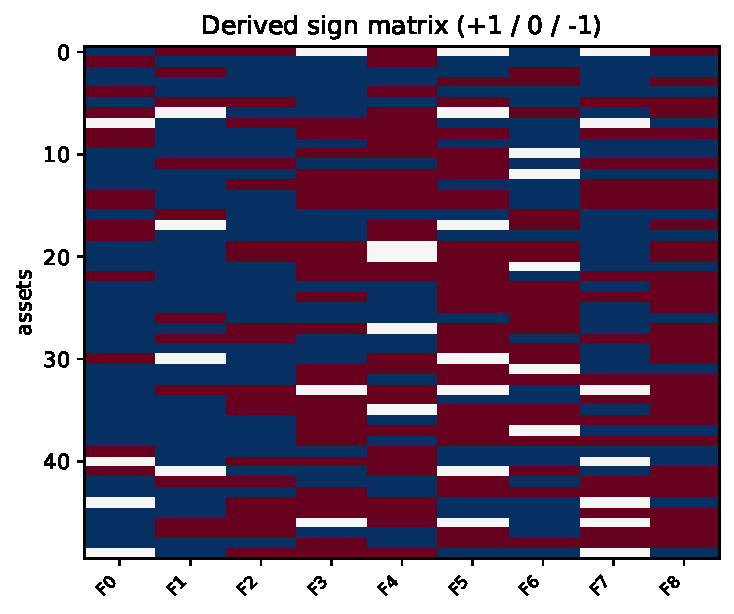
\includegraphics[width=0.6\textwidth]{figures/usage_signs_heatmap}
\caption{\label{fig:usage-signs} Gated sign matrix abstains on 34 of 450
cells. The figure renders \protect\code{derived\_signs\_} for the synthetic HCGL
fit of Section~\ref{sec:usage-example} through \protect\code{plot\_signs}. Each row is
one of the $N = 50$ responses and each column one of the $M = 9$ factors.
Blue cells carry a $+1$ sign constraint and red cells a $-1$ constraint.
The $34$ white cells are the entries that the noise-floor gate pins to
zero. Data: synthetic panel, generator seed $0$.}
\end{figure}

%% -- Comparison ---------------------------------------------------------------

\section{Comparison with existing packages} \label{sec:comparison}

This section positions \pkg{factorlasso} against six existing
sparse-regression packages spanning the \proglang{Python} and
\proglang{R} ecosystems: \pkg{scikit-learn}'s \code{Lasso} class
\citep{Pedregosa+etal:2011}, \pkg{gglasso} \citep{Yang+Zou:2015},
\pkg{sparsegl} \citep{Liang+Cohen+SolonHeinsfeld+Pestilli+McDonald:2024}, \pkg{asgl}
\citep{Mendez-Civieta+Aguilera-Morillo+Lillo:2021}, \pkg{celer}
\citep{Massias+Gramfort+Salmon:2018},
and \pkg{adelie}
\citep{Yang+Hastie:2024}. The comparison is on fifteen feature
dimensions covering both algorithmic capabilities and the software
conveniences that matter for multi-asset factor estimation in practice.

Table~\ref{tab:comparison} reports the comparison. The dimensions are
ordered roughly by ascending specificity to the multi-asset factor
model setting. Rows 1--6 cover regularisation primitives and
penalty-family variants common to LASSO-family software, including the
univariate-guided UniLasso of \cite{Chatterjee+Hastie+Tibshirani:2025}
and the cooperative LASSO of \cite{Chiquet+Grandvalet+Charbonnier:2012}.
Rows 7--10 cover the HCGL cluster discovery, the cluster-by-factor block
penalty, the cell-level sign constraints, and the noise-floor gate. Row 11
covers the adaptive reweighting of \cite{Zou:2006} and
\cite{Wang+Leng:2008} routed through both the $\ell_1$ and group $\ell_2$ paths.
Rows 12--15 cover the software conveniences (prior centring, observation
weighting, NaN tolerance, and factor covariance assembly) that a deployed
pipeline and the replication of this study require.

\begin{table}[ht]
\centering
\small
\setlength{\tabcolsep}{4pt}
\begin{tabular}{p{5.4cm}ccccccc}
	\hline
	Feature & \pkg{sklearn} & \pkg{gglasso} & \pkg{sparsegl} & \pkg{asgl} & \pkg{celer} & \pkg{adelie} & \pkg{factorlasso} \\
	\hline
	Multi-response interface ($N \times M$ in one fit) & -- & -- & -- & -- & -- & \checkmark & \checkmark \\
	$\ell_1$ penalty (LASSO) & \checkmark & -- & \checkmark & \checkmark & \checkmark & -- & \checkmark \\
	Group $\ell_2$ penalty (group LASSO) & -- & \checkmark & \checkmark & \checkmark & -- & \checkmark & \checkmark \\
	Sparse-group mixing ($\alpha \in [0, 1]$) & -- & -- & \checkmark & \checkmark & -- & -- & \checkmark \\
	Univariate-guided fit (UniLasso) & -- & -- & -- & -- & -- & -- & \checkmark \\
	Cooperative sign-coherent groups & -- & -- & -- & -- & -- & -- & \checkmark \\
	HCGL cluster discovery (clusters found internally) & -- & -- & -- & -- & -- & -- & \checkmark \\
	Cluster-by-factor block penalty (FCGL) & -- & -- & -- & -- & -- & -- & \checkmark \\
	Sign constraints at cell level & -- & -- & -- & -- & -- & -- & \checkmark \\
	Noise-floor $t$-statistic gate & -- & -- & -- & -- & -- & -- & \checkmark \\
	Adaptive penalty reweighting & -- & -- & -- & \checkmark & -- & -- & \checkmark \\
	Prior-centred shrinkage ($\bm{\beta}^0 \neq \bm{0}$) & -- & -- & -- & -- & -- & -- & \checkmark \\
	EWMA observation weighting & -- & -- & -- & -- & -- & -- & \checkmark \\
	NaN-tolerant API & -- & -- & -- & -- & -- & -- & \checkmark \\
	Factor covariance assembly & -- & -- & -- & -- & -- & -- & \checkmark \\
	\hline
	Implementation language & \proglang{Python} & \proglang{R} & \proglang{R} & \proglang{Python} & \proglang{Python} & \proglang{Python} & \proglang{Python} \\
	\hline
\end{tabular}
\caption{\label{tab:comparison} Feature comparison of \pkg{factorlasso}
	against six sparse-regression packages in the \proglang{Python} and
	\proglang{R} ecosystems. A checkmark indicates that the feature is
	provided natively by the package. A dash indicates that the feature
	is absent or must be implemented externally by the practitioner.
	\pkg{sklearn} refers specifically to the \code{Lasso} class. The
	related \code{MultiTaskLasso} class supplies a different multi-response
	formulation that enforces shared sparsity pattern rather than the
	multi-response factor model fit of \pkg{factorlasso}. This feature
	table and the empirical benchmark of
	Section~\ref{sec:sim-calibrated} cover different package sets by
	design. The benchmark runs \pkg{scikit-learn}, \pkg{skglm}, \pkg{asgl}, and \pkg{adelie} as per-asset estimators with OLS as the unregularised reference: the comparators that are installable in one
	\proglang{Python} environment and that map onto the per-asset fit
	the benchmark contrasts against. \pkg{skglm} is the benchmarked
	group-LASSO comparator and is omitted from this capability table
	only to keep the columns to the canonical six, while \pkg{celer} and \pkg{gglasso} are shown here for capability coverage but are not run, and the \proglang{R}-only \pkg{sparsegl}
	is a registered stub whose cross-language bridge is deferred to
	future work, so it is not part of the benchmark.}
\end{table}

Several dimensions in Table~\ref{tab:comparison} merit elaboration
because the operational cost of working around them in a deployed
pipeline is the implicit motivation for the \pkg{factorlasso} package.

\paragraph{HCGL cluster discovery.}
The data-driven Ward-linkage partition described in
Section~\ref{sec:hcgl} is the feature that most distinguishes
\pkg{factorlasso} from the other packages. Every package with group LASSO functionality
(\pkg{gglasso}, \pkg{sparsegl}, \pkg{asgl}, \pkg{adelie}) requires the
practitioner to supply the group structure as an external input. In
multi-asset settings the appropriate group structure is rarely known
a priori. Asset-class taxonomies provide a starting point but mask
within-class heterogeneity and the regime-dependent restructuring of
correlations under stress, when historically uncorrelated asset
classes collapse into a single risk-on factor. Requiring the
practitioner to choose groups upstream creates a tunable
hyperparameter that the methodology of this paper eliminates: clusters
are discovered from $\operatorname{corr}(\bm{Y})$, the cluster-pooled
sign derivation operates on the same partition, and the row
aggregation in the adaptive group penalty
(Equation~\ref{eq:adapt-row}) uses the same partition again. The
single-partition coherence of Section~\ref{sec:hcgl} is what gives
the package its substantive coherence rather than a collection of
independently-tunable components.

\paragraph{Cluster-by-factor block penalty.}
On the discovered partition \pkg{factorlasso} offers two group penalties
that differ in which axis of the loading matrix the norm groups. The
row-grouped penalty (HCGL) takes the $\ell_2$ norm over each asset's factor
loadings. The cluster-by-factor penalty (FCGL,
Equation~\ref{eq:fcgl}) takes the $\ell_2$ norm over the loadings of a
cluster's assets on each factor, so the cluster is the group of the norm
itself. The second grouping is intrinsically multi-response: it couples
several assets inside one norm and cannot be expressed in a
single-response solver. Every group-LASSO comparison package
(\pkg{gglasso}, \pkg{sparsegl}, \pkg{asgl}, \pkg{adelie}) groups over the
features of one response, so none can represent the cluster-by-factor
block even when run per asset. The two modes are reported as
alternatives in Section~\ref{sec:sim-calibrated}.

\paragraph{Cell-level sign constraints with a noise-floor gate.}
None of the six comparison packages implements cell-level sign
constraints. The closest published mechanism is the univariate-guided
sparse regression of \cite{Chatterjee+Hastie+Tibshirani:2025}, which
operates on a single response and does not address the noise-floor
problem at all. The closed-form SSR identity of Equation~\ref{eq:ssr}
that drives the gate, and the cluster aggregation of
Equation~\ref{eq:slope-cluster}, are developed in the companion
methodology paper \citep{Sepp+Kastenholz:2026sign}.
These mechanisms produce the within-cluster
sign coherence that an unconstrained group LASSO does not, with
empirical evidence in Section~\ref{sec:simulation} that the coherence
rises from approximately $0.36$ to $0.81$ when the mechanism is
engaged on cleanly-signed cluster data.

\paragraph{Univariate-guided and cooperative modes.}
Two of the published methods that \pkg{factorlasso} offers as
configurations bear directly on sign handling. The univariate-guided
UniLasso of \cite{Chatterjee+Hastie+Tibshirani:2025} keeps each loading on
the sign of its univariate slope unconditionally, with no noise-floor test,
and fits each response separately. The cooperative LASSO of
\cite{Chiquet+Grandvalet+Charbonnier:2012} encourages the members of a group
to share a sign through a split positive-negative penalty, a soft coherence
the data can overrule. The gated cluster-pooled mechanism of this package
differs from both: it pools the sign evidence across cluster members,
applies the noise-floor gate so that weak-evidence cells abstain rather than
inherit a sign, and then enforces the surviving signs as hard constraints.
Offering all three behind one interface lets a practitioner move between
unconditional, soft, and gated sign handling without changing the estimation
framework.

\paragraph{Prior-centred regularisation.}
Shrinkage toward a non-zero prior $\bm{\beta}^0$ is absent from every
comparison package: all six shrink toward zero, recovering the OLS
estimate in the unregularised limit. For an unconstrained penalty this
is a convenience gap rather than a capability gap: re-centring the
response (fitting $\bm{Y} - \bm{X}\,{\bm{\beta}^{0}}^{\top}$ with
zero-centred shrinkage and adding $\bm{\beta}^0$ back) reproduces
prior-centred estimation exactly. The emulation fails precisely where
this package operates. Under the cell-level sign matrix, the constraint
of Equation~\ref{eq:sgl-sign-constraint} becomes a per-cell shifted
bound on the centred coefficients, which none of the comparison solvers
accepts, so a prior cannot be combined with sign constraints from
outside the optimisation problem. The remaining workaround, post-hoc
add-back adjustments to the fitted loadings, such as forcing a positive
credit beta for high-yield assets whose sample correlation sits below
the noise floor, compromises the alpha-beta consistency that the
framework is designed to enforce by construction, since the modified
loadings no longer satisfy the optimisation problem of
Equation~\ref{eq:sgl-sign} and the implied covariance
$\hat{\bm{\beta}}\, \bm{\Sigma}_F\, \hat{\bm{\beta}}^\top + \bm{D}$
no longer corresponds to the same $\hat{\bm{\beta}}$.

\paragraph{EWMA weighting, NaN tolerance, factor covariance assembly.}
These software conveniences can in principle be implemented around any
existing package via pre- or post-processing layers. The cost of doing
so is that the pre-processing diverges between teams and between
projects, and reproducibility relies on the pre-processing being
described accurately in the methods section of every downstream
publication. \pkg{factorlasso} embeds all three at the API boundary,
producing a single artefact that handles the full pipeline from
NaN-bearing return panels with heterogeneous inception dates to a
serialisable factor covariance dataclass with persistent sign-matrix
audit trail.

\bigskip

The combinatorial pattern in Table~\ref{tab:comparison} is the point.
No single column covers all fifteen rows. The closest in coverage are
\pkg{sparsegl} (covering rows 1--4 with the inclusion of group LASSO
and sparse-group mixing) and \pkg{asgl} (covering rows 1--4 and 8
with the addition of adaptive reweighting), but both require external
group inputs and lack sign constraints. The combinatorial gap that
spans rows 5--7 and 9--13 simultaneously is what \pkg{factorlasso}
fills.

The expressiveness carries a measured runtime cost, which
Table~\ref{tab:timing} quantifies across panel widths at the
dimensions of the application in
Section~\ref{sec:application-etf} ($T = 112$, $M = 9$). The
per-asset competitors scale linearly in $N$, because they solve $N$
independent fits. The \pkg{factorlasso} fit grows
superlinearly because \pkg{CVXPY} assembles the $N$ per-asset cone
problems into one monolithic programme and the interior-point solver
does not exploit their block-separable structure. Under the full production configuration it completes
in under five seconds at $N = 500$. It runs well below \pkg{asgl} (the
only competitor with adaptive reweighting) at the smaller panel widths
(roughly a quarter of its time at $N = 50$ and $N = 100$) and is
comparable to it at $N = 500$ (around $4.5$ against $4.0$ seconds).
The FCGL block penalty matches the HCGL row penalty in wall-clock at
every width (within two percent at $N = 500$): the coupling across a
cluster's assets adds cone constraints of the same order as the
row-grouped norm, so the loss of block-separability changes how the
problem is reasoned about but not its solve time at these dimensions.
The compiled \pkg{skglm} loop is faster in absolute terms by a
factor of three to four at the smaller widths and a factor of
fourteen at $N = 500$.
For the monthly and quarterly re-estimation cycles in 
production, where one fit per currency frame is required, the
premium buys the constraint machinery of
Table~\ref{tab:comparison} at interactive speed.

\begin{table}[ht]
\centering
\begin{tabular}{lrrr}
	\hline
	Estimator & $N = 50$ & $N = 100$ & $N = 500$ \\
	\hline
	\pkg{scikit-learn} \code{Lasso} (per asset) & 0.01 & 0.03 & 0.13 \\
	\pkg{skglm} group LASSO (per asset)         & 0.03 & 0.06 & 0.31 \\
	\pkg{asgl} SGL (per asset)                  & 0.41 & 0.80 & 3.97 \\
	\code{FL LASSO} (joint)                     & 0.04 & 0.09 & 0.74 \\
	\code{FL HCGL+SIGN+ADAPT} (joint)           & 0.10 & 0.23 & 4.45 \\
	\code{FL FCGL+SIGN+ADAPT} (joint)           & 0.10 & 0.22 & 4.53 \\
	\code{FL SGL+SIGN+ADAPT} (joint)            & 0.10 & 0.23 & 4.58 \\
	\hline
\end{tabular}
\caption{\label{tab:timing} Per-asset competitors scale linearly in
	panel width, and the joint production fit grows superlinearly but
	stays under five seconds at $N = 500$. Median wall-clock seconds
	per fit over three repeats after one discarded warm-up fit
	(\pkg{skglm} JIT-compiles on first call), on synthetic panels with
	$T = 112$, $M = 9$, at $\lambda / \lambda_{\max} = 0.02$. Each entry
	is the total time for the full $N$-asset panel: the per-asset
	competitors fit the $N$ assets in an independent loop, the joint
	\pkg{factorlasso} rows in one solve under the production
	configuration of Table~\ref{tab:lassomodel-params}. Measured on the
	fourteen-core Windows~11 workstation of
	Appendix~\ref{app:reproduction}; absolute values are
	hardware-dependent, the relative ordering and scaling are the point.
	Produced by \code{simulations/timing\_scaling.py}.}
\end{table}


%% -- Simulation study ---------------------------------------------------------

\section{Simulation study} \label{sec:simulation}

This section reports a simulation study designed to quantify where the
cluster-pooled sign-derivation mechanism of Section~\ref{sec:methods}
delivers gains over the standard sparse and group LASSO baselines.
The study is run on synthetic panels generated from the harness of
Appendix~\ref{app:reproduction}, with regime parameters chosen to span the
operating envelope of multi-asset factor estimation and several
robustness directions besides. Each estimator row corresponds to one
constructor option of Section~\ref{sec:lasso-model}. The exhibits
therefore validate the software's design choices, not a new
statistical methodology.

\subsection[Study design]{Study design} \label{sec:sim-design}

The data-generating process produces synthetic panels
$\bm{Y} = \bm{X}\, \bm{\beta}_{\mathrm{true}}^\top + \bm{\varepsilon}$
with controllable sample length $T$, asset count $N$, factor count $M$,
true cluster count $K$, sign-mix regime (clean, mixed, or
idiosyncratic), sparsity level, signal-to-noise ratio (SNR), and factor
and residual covariance structure. The cluster templates are built so
$\bm{\beta}_{\mathrm{true}}$ has within-cluster sign coherence. This
coherence is degraded under the \emph{mixed} regime (a subset of cells
flipped) and removed entirely under the \emph{idiosyncratic} regime
(every active cell flipped with probability one-half). The full study
covers nineteen regimes. The regime axes abstract the qualitative
features of the fitted multi-asset model of
Section~\ref{sec:sim-calibrated}: clustered loadings, within-group sign
agreement, and the factor collinearity that misattributes a
weakly-identified exposure. The synthetic study varies these features in
isolation, while Section~\ref{sec:sim-calibrated} draws the data-generating
process from the fitted exchange-traded-fund universe directly. The grid
is a core $2\times2\times2$ ablation over 
sparse/dense $\times$ low/high-SNR $\times$ clean/mixed plus
centre points, three sample-length stress points
$T \in \{60, 120, 240\}$, an $N = 200$ scaling regime, cluster-count and
covariance-structure robustness regimes, crossed with five seeds, six
estimators, and five $\lambda$ values, a 2{,}850-cell grid. The full grid
is available in the per-cell replication outputs documented in
Appendix~\ref{app:reproduction}. This
section summarises the findings that bear on when to use the mechanism.

\begin{sloppypar}
Six \pkg{factorlasso} configurations form a strict ablation:
\code{LASSO} (cellwise $\ell_1$, no groups, no signs), \code{GRP-ORACLE}
(group LASSO with true cluster labels supplied, the unattainable best
case), \code{GRP-HCGL} (group LASSO with HCGL-discovered clusters),
\code{+SIGN} (HCGL plus the gated cluster-pooled sign derivation),
\code{+SIGN+ADAPT} (plus adaptive group-$\ell_2$ reweighting), and
\code{SGL+SIGN+ADAPT} (plus a partially active cellwise $\ell_1$ path at
\code{l1_weight}~$=0.1$, the most fully-featured configuration). The
\code{LASSO} and \code{GRP-ORACLE} rows bracket the contribution: any
gain over \code{LASSO} is attributable to group structure, and any gain
of HCGL-plus-signs over \code{GRP-ORACLE} to the sign mechanism rather
than to cluster information per se. Each fit is scored on support
recovery $F_1$, sign-agreement rate, normalised
$\beta$-MSE ($\|\hat{\bm{\beta}} - \bm{\beta}_{\mathrm{true}}\|_F^2$
divided by $\|\bm{\beta}_{\mathrm{true}}\|_F^2$),
cluster sign coherence (the fraction of true-cluster/factor pairs whose
non-zero fitted coefficients share a sign), and factor risk-premium
RMSE. For each (regime, seed, estimator) triple the reported row is the
$\lambda$ minimising $\beta$-MSE (oracle selection, used to isolate the
estimator-level question from $\lambda$-selection, which is not this
paper's contribution).
\end{sloppypar}


\subsection[Headline ablation]{Headline ablation} \label{sec:sim-headline}

Table~\ref{tab:headline-ablation} reports the mean of each metric across
all nineteen regimes and five seeds at the oracle-selected $\lambda$. The
headline pattern is in the coherence column: the three sign-derivation
rows (\code{+SIGN}, \code{+SIGN+ADAPT}, \code{SGL+SIGN+ADAPT}) reach
cluster sign coherence of approximately $0.68$ ($0.677$ to $0.685$), roughly twice the
$0.29$ to $0.36$ of the three unconstrained rows. The mechanism
delivers the within-cluster sign coherence it is designed to deliver,
and the coherence separation is many standard errors wide (SE
$\approx 0.014$ on a gap of $0.39$). On
normalised $\beta$-MSE the fully-featured \code{SGL+SIGN+ADAPT} edges the
unconstrained baselines ($0.346$ versus $0.366$ for \code{LASSO} and
$0.495$ for \code{GRP-HCGL}), but the margin over \code{LASSO} is within
the combined standard error and should not be read as a decisive
averaged improvement. The averaged margin is modest because it
mixes regimes where the mechanism wins decisively with regimes where it
adds bias, a cross-section the next subsection isolates.

\begin{table}[ht]
\centering
\small
\setlength{\tabcolsep}{4pt}
\begin{tabular}{lrrrrr}
	\hline
	Estimator & Support $F_1$ & Sign rate & $\beta$-MSE & Coherence & Risk-premium RMSE \\
	\hline
	\code{LASSO}            & 0.657 (0.002) & 0.968 (0.003) & 0.366 (0.011) & 0.358 (0.004) & 0.068 (0.004) \\
	\code{GRP-ORACLE}       & 0.591 (0.000) & 0.978 (0.002) & 0.434 (0.013) & 0.290 (0.005) & 0.069 (0.004) \\
	\code{GRP-HCGL}         & 0.591 (0.000) & 0.977 (0.002) & 0.495 (0.017) & 0.288 (0.006) & 0.071 (0.004) \\
	\code{+SIGN}            & 0.697 (0.002) & 0.906 (0.004) & 0.367 (0.005) & 0.679 (0.014) & 0.073 (0.003) \\
	\code{+SIGN+ADAPT}      & 0.695 (0.002) & 0.907 (0.004) & 0.358 (0.005) & 0.677 (0.014) & 0.072 (0.003) \\
	\code{SGL+SIGN+ADAPT}   & 0.704 (0.002) & 0.905 (0.005) & 0.346 (0.005) & 0.685 (0.014) & 0.072 (0.003) \\
	\hline
\end{tabular}
\caption{\label{tab:headline-ablation} Headline ablation: mean of each
	metric across all nineteen regimes and five seeds at oracle-selected
	$\lambda$, with the standard error across seeds in parentheses. Support
	$F_1$ is the F1 score of the non-zero-versus-zero
	classification of the loading cells, and sign rate is the fraction of
	true-non-zero cells with correctly signed estimates. Higher is better
	for support $F_1$, sign rate, and coherence.
	Lower is better for $\beta$-MSE and risk-premium RMSE.}
\end{table}

The sign-derivation rows score lower on sign rate ($\approx 0.91$
versus $0.97$ to $0.98$), a shrinkage artefact rather than a failure:
the sign-rate metric is conditional on a truly non-zero cell, so a
true-support cell the gate pins to zero counts as a mismatch even
though it is zeroed, not wrong-signed. The same gate raises support
$F_1$ from $0.59$ to $0.70$.


\subsection[Where the mechanism wins]{Where the mechanism wins} \label{sec:sim-core}

The core $2 \times 2 \times 2$ ablation crosses sparsity (sparse/dense),
signal-to-noise (low/high), and sign coherence (clean/mixed), with the
idiosyncratic regime excluded as out of scope. Normalised $\beta$-MSE
across these cells is regime-dependent: the sign mechanism helps most
when the truth is sparse and the signal is weak, adds modest overhead
when the signal is strong and sparse, and adds bias when the truth is
dense and the signal strong (the standard sparsity-method failure mode).
In the most favourable panel (sparse + low-SNR, clean signs)
\code{SGL+SIGN+ADAPT} reaches $\beta$-MSE $0.54$ against \code{GRP-HCGL}'s
$0.97$, a reduction of roughly forty-four percent against that baseline.
In the dense + high-SNR panel the unconstrained estimators win. The
regime where the mechanism operates most usefully is precisely the
sparse-to-moderate, low-SNR, short-sample regime that multi-asset capital
market assumption (CMA) estimation occupies. The advantage is largest at
$T = 60$ and persists in attenuated form to $T = 240$, as the $T$ slices
of the calibrated benchmark (Table~\ref{tab:competitor}) confirm.

The complementary safety property is that the mechanism does not fabricate
structure absent from the data. In the idiosyncratic regime, where every
active sign is independently flipped so the truth has essentially no
within-cluster coherence, the sign-derivation output coherence falls to
approximately $0.17$ (against $0.81$ in the clean regime). A practitioner
applying the mechanism to data where the within-cluster sign assumption
does not hold gets a near-zero gate output and a fit that tracks the
unconstrained baseline, not spurious constraints.


\subsection[Discussion]{Discussion} \label{sec:sim-discussion}

\textbf{HCGL is a sign-coherent grouping method, not a cluster recovery
method.} The
adjusted Rand index between HCGL-discovered clusters and the true
clusters sits at approximately $0.23$ across all regimes (well above
zero but well below the oracle $1.0$), while within-cluster sign
coherence on the HCGL partition reaches approximately $0.81$ in the
clean regime. The discovered clusters do not match the data-generating
partition, but their members share signs on their dominant factors,
which is the only property the downstream sign derivation needs. The
distinction is the one drawn in the clustering-stability literature
between accuracy (agreement with a ground-truth partition, which ARI
measures) and replicability (agreement of the partition under
resampling), the latter being the assessable criterion when no ground
truth exists \citep{vonLuxburg:2010}. In the deployed
setting a resampling-based replicability assessment in the spirit of
\citet{Sorooshyari+Rivas+Tibshirani:2026} is the appropriate diagnostic
and is left to applied work.

Density and signal-to-noise are
not knowable a priori, so the operational rule is selector-based: fit
with and without the constraints and compare on the practitioner's own
criterion (BIC or cross-validation), and disable the constraints when
the unconstrained fit wins. Two observable signals support the choice.
A high gate-abstention rate indicates weak within-cluster sign evidence,
where the mechanism is inert rather than harmful. Instability of the
derived sign matrix under resampling the panel indicates that the pooled
signs are not reproducible and should not be imposed as hard
constraints.


\subsection[Calibrated multi-asset benchmark]{Calibrated multi-asset
benchmark against competing packages} \label{sec:sim-calibrated}

The ablation above isolates the sign mechanism on synthetic templates.
This subsection asks the complementary question a practitioner cares
about: on a data-generating process calibrated to a real multi-asset
universe, with the true loadings known, does the full \pkg{factorlasso}
stack (including the economic prior) improve on the competing
sparse-regression packages? We calibrate the DGP to the publicly reproducible $102$-asset ETF
universe of Section~\ref{sec:application-etf}, $N = 102$ funds across
eighteen sub-asset classes loaded on the $M = 9$ macro factors of the
MATF-CMA framework, enumerated in full in
Section~\ref{sec:application-etf-data}.

Each fund's true loading vector starts from the published
sub-asset-class loading profile that the fund proxies
\citep{Sepp+Hansen+Kastenholz:2026MATF}: each exchange-traded fund is
mapped to the sub-asset class it represents (regional equity,
investment-grade credit, and so on), and takes that class's
representative loadings as its baseline. We perturb each nonzero loading
by independent Gaussian multiplicative noise with a fifteen percent
relative standard deviation, fixed per fund, which preserves the
sub-class zero pattern while giving the funds in a cluster distinct
loading magnitudes. The perturbation breaks the exact within-cluster
identity that the synthetic templates impose, so the calibrated panel
tests cluster recovery against genuinely heterogeneous members. The factor covariance is the sample covariance of
the nine factor-return series over the panel window. It carries a
credit--equity factor correlation of $0.84$, the near-collinearity that
makes the credit loading statistically fragile to identify. Idiosyncratic
variances are set per fund to reproduce that fund's empirical
ordinary-least-squares $R^2$, and the true clusters are the eighteen
sub-asset classes. Each replication draws a training window and an
equal-length test window. The base sample is $T = 112$ months, with
$T \in \{60, 240\}$ as the small- and large-sample stress points.

The roster pairs five competitors against the sign-and-prior
configuration. The competitors are ordinary least squares,
\pkg{scikit-learn}'s per-asset \code{Lasso}, \pkg{skglm}'s group LASSO, \pkg{asgl}'s sparse group LASSO, and \pkg{adelie}'s group LASSO,
each applied per asset on the same coefficient geometry. They run
against the \pkg{factorlasso} ladder of Section~\ref{sec:sim-design} and two
economically-constrained configurations the competitors cannot express:
\code{HCGL+PRIOR}, which centres the credit loadings of the IG, HY and
EM sleeves on prior values of $0.20$, $0.40$ and $0.30$, and
\code{HCGL+SIGN+PRIOR}, which adds the cell-level economic sign matrix.
The clustered \pkg{factorlasso} rows run the \emph{production
configuration} of the MATF-CMA deployment
(Table~\ref{tab:lassomodel-params}): \code{cutoff\_fraction = 0.40},
gate $\tau = 1.0$, and adaptive reweighting with floor $0.5$, all set
a priori rather than tuned on this DGP. The production EWMA span is
excluded: the DGP is stationary, so time-decayed observation weights
are pure efficiency loss and would not inform the comparison.
Each estimator is tuned by two $\lambda$-selectors: \emph{oracle}, the
$\lambda$ minimising $\beta$-MSE (the most generous choice for each
competitor) and \emph{BIC}, which a practitioner can actually
compute. Alongside the statistical metrics of
Section~\ref{sec:sim-design} we score three economic quantities on the
seventeen credit-bearing (IG/HY/EM) funds: the mean recovered Credit
loading (true value $0.36$), the error in Credit's share of those funds'
systematic variance, and the relative Frobenius error of the systematic
covariance $\hat{\bm{\beta}} \bm{\Sigma}_F \hat{\bm{\beta}}^\top$.

\begin{table}[ht]
\centering
\small
\setlength{\tabcolsep}{4.5pt}
\begin{tabular}{lrrrrrrr}
	\hline
	Estimator & $\beta$-MSE & Supp.\ $F_1$ & Sign agr. & OOS $R^2$ & Credit $\beta$ & Risk-sh.\ err & Cov err \\
	\hline
	OLS                              & 0.620 & 0.657 & 0.891 & 0.672 & 0.350 & 0.073 & 0.123 \\
	\pkg{scikit-learn} \code{Lasso}  & 0.216 & 0.677 & 0.544 & 0.642 & 0.009 & 0.406 & 0.166 \\
	\pkg{skglm} group LASSO          & 0.268 & 0.657 & \textbf{0.923} & 0.651 & 0.078 & 0.307 & 0.152 \\
	\pkg{asgl} SGL                   & 0.242 & 0.670 & 0.906 & 0.639 & 0.064 & 0.320 & 0.169 \\
	\pkg{adelie} group LASSO         & 0.276 & 0.657 & 0.922 & 0.642 & 0.078 & 0.306 & 0.163 \\
	\code{FL LASSO}                  & 0.219 & 0.724 & 0.652 & 0.663 & 0.036 & 0.374 & 0.137 \\
	\code{FL HCGL+SIGN+ADAPT}        & 0.224 & 0.689 & 0.843 & 0.662 & 0.089 & 0.295 & 0.137 \\
	\code{FL FCGL+SIGN+ADAPT}        & 0.188 & 0.733 & 0.808 & 0.681 & 0.151 & 0.233 & 0.120 \\
	\code{FL SGL+SIGN+ADAPT}         & 0.218 & 0.698 & 0.834 & 0.659 & 0.088 & 0.294 & 0.141 \\
	\code{FL HCGL+SIGN+PRIOR}        & 0.185 & 0.731 & 0.848 & 0.663 & 0.319 & 0.127 & 0.140 \\
	\code{FL FCGL+SIGN+PRIOR}        & \textbf{0.161} & \textbf{0.773} & 0.811 & \textbf{0.683} & 0.309 & \textbf{0.071} & \textbf{0.119} \\
	\code{FL ORACLE+SIGN+PRIOR}      & 0.204 & 0.736 & 0.844 & 0.659 & \textbf{0.322} & 0.102 & 0.137 \\
	\hline
\end{tabular}
\caption{\label{tab:competitor} Calibrated multi-asset benchmark at
	oracle-selected $\lambda$, sample $T = 112$, mean over fifteen seeds.
	\code{FL} denotes \pkg{factorlasso}. The competitor packages are applied
	per asset. Lower is better for $\beta$-MSE, risk-share error, and
	covariance error, and higher is better for support $F_1$, sign agreement (fraction of
	true-non-zero cells with correctly signed estimates), and OOS $R^2$. The
	true Credit loading on the credit-bearing funds is $0.36$. Bold marks the
	column-best among estimators with non-degenerate fit. Standard
	errors across the fifteen seeds on the two discriminating columns are
	small: $\beta$-MSE standard errors fall in $0.004$ to $0.026$ and
	Credit $\beta$ standard errors in $0.001$ to $0.009$ across the rows.
	The credit-recovery gap between the prior
	configuration and the best competitor exceeds fifty standard errors
	of the difference. The full ladder,
	the BIC operating points, and the $T \in \{60, 240\}$ slices are produced
	by the reproduction scripts of Appendix~\ref{app:reproduction}.}
\end{table}

At oracle $\lambda$ the packages are statistically close
(Table~\ref{tab:competitor}): normalised $\beta$-MSE spans $0.16$ to
$0.27$ across the regularised estimators, and the two prior-centred
configurations lead the column, the FCGL mode at $0.161$ and the HCGL
mode at $0.185$.
\pkg{factorlasso}'s sign-constrained and adaptive configurations match
or edge every competing package on support $F_1$ ($0.69$--$0.70$ versus
$0.66$--$0.68$), out-of-sample $R^2$ ($0.66$ versus $0.64$--$0.65$), and
systematic-covariance error ($0.14$ versus $0.15$--$0.17$). The
sign-derivation and adaptive layers buy their structural properties
without a fit penalty, exactly as on the synthetic data. Sign agreement
with the true loadings reads differently here, and the dense calibrated
loadings explain why: the truth is dense, so every cell an $\ell_1$
penalty or the noise-floor gate zeroes is a true exposure counted as a
sign miss. \pkg{scikit-learn}'s per-asset $\ell_1$ collapses to
$0.54$, the \pkg{factorlasso} LASSO sits at $0.65$, and the gated
configurations ($\tau = 1.0$) sit at $0.83$ to $0.85$ — below the
ungated group estimators at $0.91$ to $0.92$, which zero whole groups
rarely. The column orders estimators by how much they shrink or gate,
not by economic fidelity: the metric artefact established on the
synthetic ablation, amplified by a dense truth. Runtime favours the
compiled solvers at this scale, consistent with the \pkg{CVXPY}
positioning of Section~\ref{sec:cvxpy-backend} and the scaling exhibit
of Table~\ref{tab:timing}.

The economic columns tell a different story, and it is the central one
for multi-asset CMA estimation. Against a true mean Credit loading of
$0.36$ on the seventeen credit-bearing funds, every penalised competitor recovers
at most $0.08$: under the $0.84$ credit--equity collinearity the
penalised estimators shrink the weakly-identified credit loading toward
zero and absorb the exposure into the equity factor. \pkg{scikit-learn}'s
pure $\ell_1$ zeros it outright ($0.009$). The
adaptive reweighting recovers part of it ($0.09$). Only the economic
prior recovers it in full ($0.32$), cutting the credit risk-share error
to well under half of the group-LASSO competitors' ($0.13$ against
$0.31$--$0.32$). A prior
alone is not the differentiator: re-centring the response reproduces
prior-centred shrinkage around any of these packages. What no competing
API expresses is the prior \emph{jointly} with cell-level sign
constraints and internally discovered groups. This integrated
configuration recovers the credit loading in full while attaining a
$\beta$-MSE ($0.185$) below every competing package. Ordinary least
squares also recovers the loading ($0.35$), but only by declining to
regularise, at the worst $\beta$-MSE in the table ($0.62$).

The \code{ORACLE+SIGN+PRIOR} row isolates the value of cluster
\emph{discovery}: it runs the identical sign, adaptive, and prior
machinery but pools signs over the true sub-asset-class taxonomy rather
than the HCGL-discovered partition. Discovery matches the known
taxonomy on the economic quantities (credit recovery $0.319$ versus
$0.322$, a tie within standard error) and slightly improves on
$\beta$-MSE ($0.185$ versus $0.204$), so the data-driven partition is at
least as good as a hand-maintained taxonomy as the pooling unit and
costs nothing when no taxonomy is available. The same holds without the
prior: \code{HCGL+sign+adapt} and \code{ORACLE+sign+adapt} are within
standard error on both $\beta$-MSE ($0.224$ versus $0.236$) and support
$F_1$ ($0.689$ versus $0.694$). Discovery is the convenience the package
provides, not a source of attribution error relative to the oracle
grouping.

The \code{FCGL} rows report the cluster-by-factor penalty of
Equation~\ref{eq:fcgl} under the otherwise identical sign-and-adaptive
and sign-and-prior configurations. On this calibrated DGP, in which the
true loadings share a per-sub-class centre, FCGL improves on its HCGL
counterpart on every fit and economic column: paired across the fifteen
seeds, $\beta$-MSE falls by $0.036$ without the prior and $0.024$ with
it, support $F_1$ rises by about $0.043$, out-of-sample $R^2$ by about
$0.019$, and the credit risk-share error by about $0.06$, each more than
two paired standard errors. The one column that moves the other way is
sign agreement, which falls by about $0.035$: the per-block norm zeros a
whole cluster-by-factor block at once, so a block it sets to zero counts
every member as a sign miss, the same metric artefact that the gated
estimators show against the dense truth. The two modes trade
differently against the same metrics, and the gap reflects the match
between the penalty and the data: the cluster-by-factor norm rewards a
truth whose within-cluster loadings are close, while the row norm makes
no homogeneity assumption. We report both rather than rank them, because
the ranking is a property of the application's cluster structure rather
than of the estimator. Appendix~\ref{app:reproduction} documents a sweep
over the within-cluster heterogeneity of the truth and over an
alternative ground truth centred on per-asset OLS loadings, under which
the ordering on support recovery reverses, confirming that neither mode
dominates across data-generating assumptions.

The two $\lambda$-selectors sharpen the contrast under a feasible
criterion. Because the empirical
loadings are dense, BIC (which trades fit against parameter count)
finds no sparsity to reward and selects its least-regularised grid
point, at which \pkg{skglm} and unconstrained
\pkg{factorlasso} revert \emph{exactly} to OLS ($\beta$-MSE $0.62$). Only
\pkg{factorlasso}'s sign-, adaptive-, and prior-constrained configurations
reach a genuinely regularised operating point under BIC, holding
$\beta$-MSE well below OLS ($0.27$ for the sign and adaptive
configurations, $0.24$ for the prior). On an economically dense truth the
structure, not the $\lambda$-tuning, is what lets a feasible selector
return a stable fit at all. The unstructured group methods can only
revert to the high-variance least-squares estimate. The small-sample
behaviour follows the same pattern across the $T$ slices of
Table~\ref{tab:competitor}: the prior's credit-recovery advantage is widest
at $T = 60$ (it recovers $0.32$ against the competitors' $0.06$) and
narrows only modestly by $T = 240$ (where the competitors reach
$0.12$), while $\beta$-MSE falls for every
estimator as the sample grows.

Two qualifications are owed. The prior values ($0.20/0.40/0.30$) sit
close to the calibration truth, so the credit-recovery comparison is
partly favourable by construction. But under $0.84$ collinearity the
credit loading is not identified from the panel alone, which is
precisely why OLS is unstable and every penalised competitor zeros it,
so the external prior performs necessary structural work rather than
fitting in-sample noise. And the adjusted Rand index between the
discovered clusters and the eighteen sub-asset labels is low
(approximately $0.2$), for the reason established in
Section~\ref{sec:sim-discussion}: the factor structure crosscuts the
product taxonomy (rate-sensitive bonds cluster with government bonds,
risk-on high-yield with equities), so the discovered partition is an
economic correlation grouping, not a recovery of the sub-asset names,
which is the property the downstream pooling actually requires. A prior
set near the calibration truth recovering that truth is weak evidence
on its own. A misspecification sweep that scales the credit prior across
a wide band and into the wrong sign leaves $\beta$-MSE within $0.19$ to
$0.21$ and covariance error flat at $0.13$ throughout. The sign
constraint of Equation~\ref{eq:sgl-sign-constraint} holds a wrong-signed
prior near zero ($0.04$) rather than letting it drive the loading
negative, so the prior is bounded-harmless when it is wrong.
Figure~\ref{fig:prior-sweep} plots the sweep, with the recovered loading
rising through the truth on the left and the bounded error on the right.

\begin{figure}[ht]
\centering
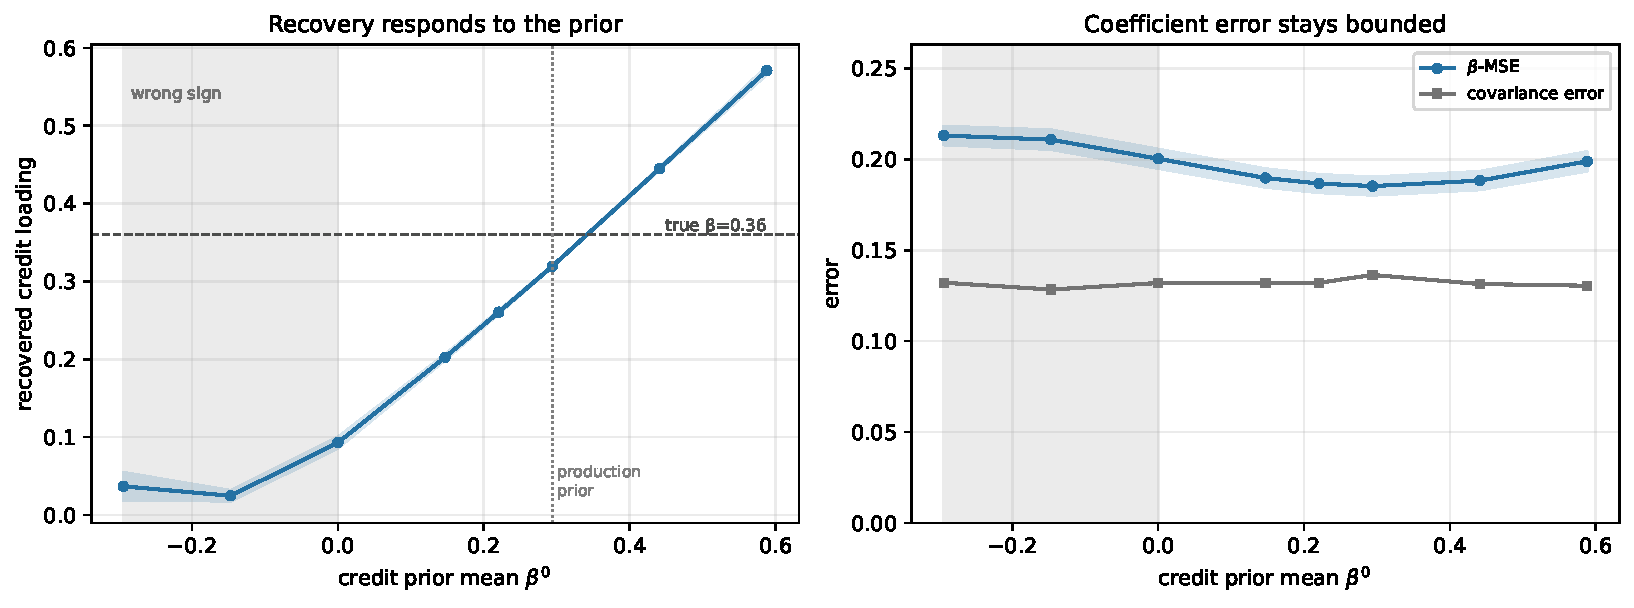
\includegraphics[width=\textwidth]{figures/prior_sensitivity_sweep}
\caption{\label{fig:prior-sweep} Prior misspecification sweep on the calibrated
$102$-asset ETF DGP at oracle-selected $\lambda$, $T = 112$, mean over fifteen
seeds with $\pm$ one standard-error bands. The credit prior mean $\beta^{0}$ is
scaled from the wrong sign (shaded) through the production value to twice the
truth. Left: the recovered credit loading rises monotonically with the prior
and crosses the calibration truth of $0.36$. Right: $\beta$-MSE and the
systematic-covariance error stay bounded across the whole band, so a
misspecified prior does not degrade the fit.}
\end{figure}

The gate threshold $\tau$ is likewise not a fragile choice.
Figure~\ref{fig:tau-sweep} sweeps it from $0$ to $3$ on the same DGP with the
production configuration otherwise fixed: support $F_1$, sign agreement, and
$\beta$-MSE are flat to within sampling error while the abstention rate rises
monotonically, so the production $\tau = 1.0$ sits on a plateau rather than a
knife-edge.

\begin{figure}[ht]
\centering
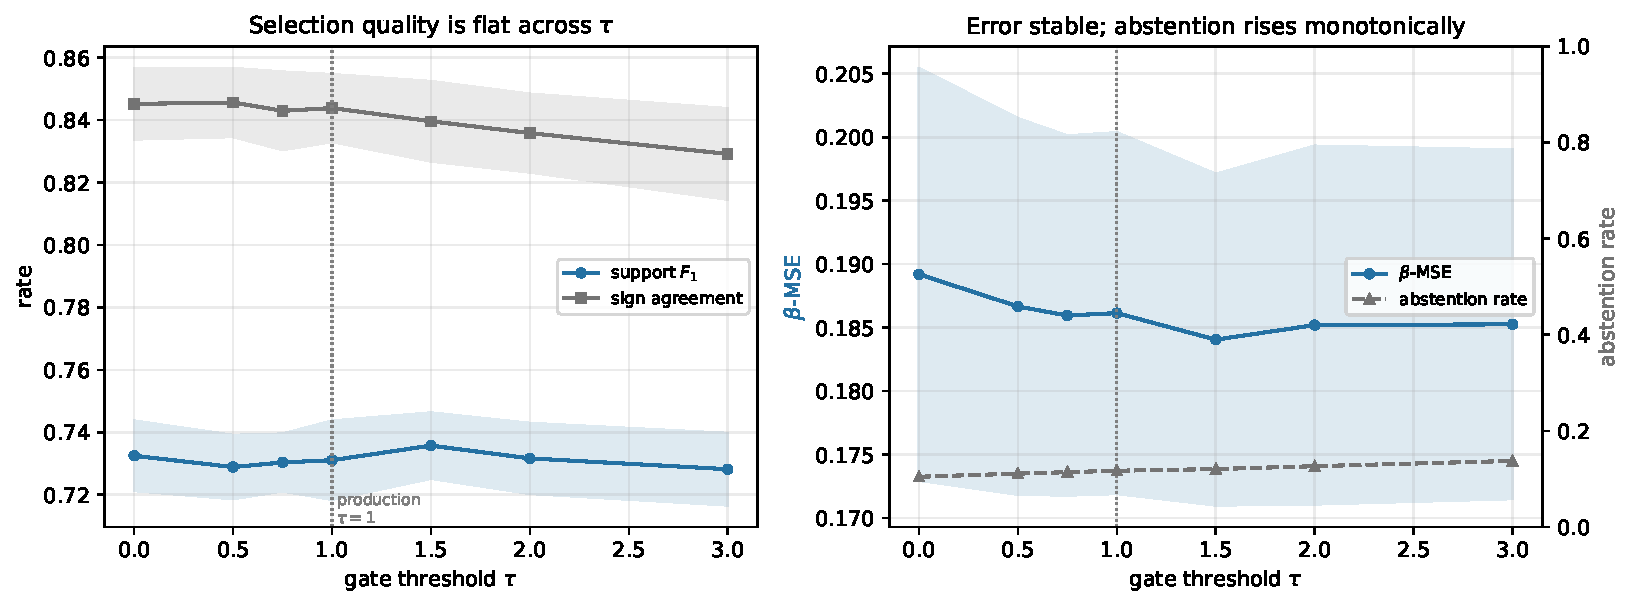
\includegraphics[width=\textwidth]{figures/tau_sweep}
\caption{\label{fig:tau-sweep} Gate-threshold sensitivity on the calibrated
$102$-asset ETF DGP, $T = 112$, mean over ten seeds with $\pm$ one
standard-error bands. The deployed HCGL+SIGN+PRIOR configuration is held fixed
and only the noise-floor threshold $\tau$ is swept; the oracle $\lambda$ is
selected once per seed at $\tau = 1.0$. Left: support $F_1$ and sign agreement
are flat across the range. Right: $\beta$-MSE stays within $0.184$ to $0.189$
while the abstention rate, the fraction of cells the gate leaves unconstrained,
rises monotonically. The production $\tau = 1.0$ sits on a plateau.}
\end{figure}

%% -- Application: multi-asset CMA ---------------------------------------------

\section[Application: multi-asset capital market assumptions]{Application:
multi-asset capital market assumptions} \label{sec:application-etf}

The deployed setting that motivates \pkg{factorlasso}, the multi-asset
allocation framework of \citet{Sepp+Ossa+Kastenholz:2026}, is capital
market assumption (CMA) estimation: the loadings of a broad
cross-section of asset-class proxies on a handful of macro factors,
used to build forward-looking risk and return assumptions. This section
runs that setting on a publicly reproducible universe to show that the
estimator behaves on market data as the calibrated simulation of
Section~\ref{sec:sim-calibrated} predicts against ground truth. This is
a demonstration of estimator behaviour, not an empirical study: real
loadings are unobservable, so the section does not claim that the
prior-centred estimates forecast better or build better portfolios than
the alternatives. The claim is the narrower one that the
misattribution the simulation diagnoses under collinearity is visible on
real data, and that the prior holds the credit loading where the
unconstrained penalty discards it. Out-of-sample predictive and
portfolio evaluation is the province of applied work using the
estimator, not of this software description.


\subsection[Data]{Data} \label{sec:application-etf-data}

The cross-section is a curated universe of $N = 102$ exchange-traded
funds spanning eighteen sub-asset classes. The fixed-income side covers
government, investment-grade, high-yield and emerging-market bonds and a
residual fixed-income sleeve. The equity side covers North American,
European, Japanese, Asia-ex-Japan and emerging-market ex-Asia equities
together with the nine US sector funds. The alternatives side covers
hedge funds, private equity and private debt, precious and non-precious
commodities, real estate, and seven currencies. The ticker list, sub-asset-class
labels, and download script (\code{fetch\_etf\_panel.py}, built on
\pkg{yfinance}, \citealp{yfinance}) ship with the package, so the panel regenerates without
a data licence and without a holdings snapshot.

Total-return adjusted prices are resampled to month-end and converted to
log returns. The thirteen-week US Treasury-bill yield is converted to a
monthly log rate and subtracted to give excess returns, matching the
convention of the macro-factor return series. Those nine factor series
(equity, rates, credit, carry, inflation, commodities, private
equity, rates volatility, and a zero-premium dollar factor) are the
excess-return factor portfolios of the CMA framework
\citep{Sepp+Hansen+Kastenholz:2026MATF}. Aligning the two yields a
balanced panel of $T = 112$ months (February~2017 through mid-2026)
$\times$ $N = 102$ funds $\times$ $M = 9$ factors. Over this window the
credit and equity factors carry a return correlation of $0.84$ (the
collinearity at the centre of the simulation), with
rates-volatility/equity at $-0.42$ and inflation/commodities at $0.72$.
All estimates in this section use the production configuration of
Table~\ref{tab:lassomodel-params} (\code{cutoff_fraction = 0.40}, gate
$\tau = 1.0$, adaptive reweighting with floor $0.5$, and the
sub-asset-class sign overlay shipped with the package) under uniform
observation weights. The production EWMA span is a non-stationarity
device and is omitted here so that the article runs one weighting
convention throughout.


\subsection[Credit attribution under shrinkage]{Credit attribution under
shrinkage} \label{sec:application-etf-credit}

We estimate the loadings under increasing regularisation and track the
credit attribution of the seventeen IG/HY/EM bond funds, instruments
that are, by construction, credit exposures. Figure~\ref{fig:etf-credit}
plots their mean Credit loading against the normalised penalty strength,
for the HCGL shrink-to-zero estimator, the prior-centred HCGL
configuration, and the prior-centred FCGL configuration, with the
unregularised ordinary-least-squares estimate as reference.

The ordinary-least-squares mean Credit loading is $0.82$. As the penalty
strengthens, the shrink-to-zero estimator drives it to zero and reassigns
the exposure to equity (whose mean loading on these funds rises from
approximately zero to $0.11$ at a moderate penalty), the
misattribution the calibrated benchmark
of Section~\ref{sec:sim-calibrated} diagnoses against ground truth. The
prior-centred estimator instead holds the loading at its economic prior
(a sleeve-weighted target of $0.29$) across the entire path. The
prior-centred FCGL estimator retains more credit attribution than this
under shrinkage: its cluster-by-factor penalty shrinks each sleeve's
deviation from the prior as a block, so the high-signal high-yield and
emerging-market sleeves stay above the prior while the low-signal
investment-grade sleeve settles at it. The per-fund picture is the same
at a moderate penalty: the Credit loading of HYG collapses from $0.85$ to $0.04$ while the prior
holds it at $0.41$. EMB collapses from $1.16$ to $0.08$ against a
prior-held $0.35$, and LQD from $0.60$ to $0.04$ against $0.22$.

\begin{figure}[!htbp]
\centering
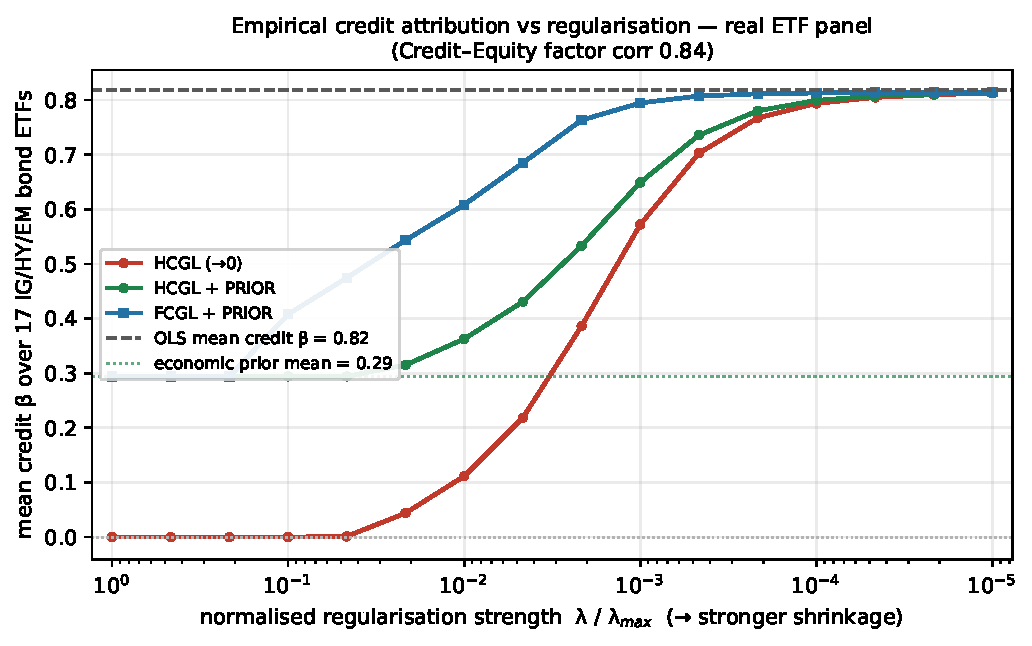
\includegraphics[width=0.85\textwidth]{figures/etf_credit_beta_vs_lambda}
\caption{\label{fig:etf-credit} Mean Credit loading of the seventeen
	IG/HY/EM bond ETFs against normalised regularisation strength
	$\lambda / \lambda_{\max}$ (stronger shrinkage to the left), on the
	$2017$--$2026$ excess-return panel. The shrink-to-zero HCGL estimator
	(red) collapses the credit attribution to zero, absorbing it into the
	equity factor. The prior-centred HCGL estimator (green) holds it near the
	economic prior. The prior-centred FCGL estimator (blue) retains more
	credit attribution under shrinkage, because its cluster-by-factor penalty
	keeps the high-signal high-yield and emerging-market sleeves above the
	prior rather than pulling every sleeve to it. The dashed line marks the
	unregularised OLS mean Credit loading, $0.82$.}
\end{figure}

This is the simulation result of Section~\ref{sec:sim-calibrated} in
market data, and it carries the same reading. There is no ground-truth
loading to recover here, but the behaviour is unambiguous: an
unconstrained penalty asked to attribute risk across collinear macro
factors zeros the credit factor on instruments that are definitionally
credit and books the exposure as equity, and no penalty strength repairs
it. For a CMA engine whose downstream consumers decompose portfolio risk
by factor, the economic prior is what holds the attribution in place.


%% -- Summary ------------------------------------------------------------------

\section{Summary and discussion} \label{sec:summary}

The \pkg{factorlasso} package supplies a sparse multi-response factor
model estimator with a cluster-pooled sign-derivation layer no single
existing package provides. The methodology of Section~\ref{sec:methods}
combines four ingredients not found together in published software:
hierarchical clustering group LASSO discovery of asset clusters,
cluster-pooled univariate slopes filtered by a closed-form noise-floor
$t$~statistic, the derived sign matrix enforced as hard convex
constraints inside a CVXPY sparse group LASSO, and Zou--Wang--Leng
adaptive reweighting on both penalty paths. The package is deployed in a
multi-asset allocation framework \citep{Sepp+Ossa+Kastenholz:2026} for
quarterly capital market assumption estimation
\citep{Sepp+Hansen+Kastenholz:2026MATF}.

The simulation study of Section~\ref{sec:simulation} reports three
findings. The cluster-pooled sign mechanism delivers the within-cluster
sign coherence it targets, from approximately $0.36$ on the
unconstrained baselines to approximately $0.81$ on cleanly-signed
cluster data. The accuracy gain concentrates in the small-sample,
low-SNR, sparse-loadings regime that capital market assumption
estimation occupies: in the most favourable panel the reduction in
normalised $\bm{\beta}$-MSE against the unconstrained group LASSO is
roughly forty-four percent, with the margin
over plain LASSO regime-specific rather than uniform. And the mechanism
is self-aware: on the idiosyncratic regime where the within-cluster sign
assumption is broken by construction, output coherence falls to
approximately $0.17$ rather than a fabricated value, so the mechanism
abstains when the data do not support it.

The calibrated multi-asset benchmark of Section~\ref{sec:sim-calibrated}
adds what the synthetic ablation cannot reach. On a data-generating
process matched to the $102$-fund ETF universe with the true loadings
known, \pkg{factorlasso}'s constrained configurations match
\pkg{scikit-learn}, \pkg{skglm}, and \pkg{asgl} on support recovery,
out-of-sample $R^2$, and systematic-covariance error, so the structural
machinery costs nothing in generic accuracy. But under the $0.84$
credit--equity collinearity the universe carries, every competing
package and every unconstrained configuration shrinks the
weakly-identified credit loading toward zero and absorbs it into equity,
while the sign- and prior-constrained configuration alone recovers it
($0.32$ against a true $0.36$, versus at most $0.08$ for the
competitors). The capability gap is the integrated estimator: a prior
can be re-centred around any package, but not jointly with cell-level
sign constraints. The same pattern appears directly in the market-data
application of Section~\ref{sec:application-etf}.

\paragraph{Practical recommendations.}
The full \code{SGL+SIGN+ADAPT} configuration is the default in the
financial-panel regime of short samples, sparse loadings, and low
signal-to-noise (Section~\ref{sec:sim-discussion}). The operational rule
is selector-based: where density and signal strength are not known a
priori, fit with and without the gate and disable it
(\code{auto_sign_constraints = False}) when a selector prefers the
unconstrained fit. The safety property makes this low-risk, since on
data without within-cluster sign coherence the derived constraints are
near-trivial and the fit tracks the unconstrained baseline.

\paragraph{Limitations.}
The noise-floor threshold is held at its default $\tau = 0.75$ across the
synthetic ablation while the calibrated benchmark and application run the
deployed $\tau = 1.0$; a theoretically optimal $\tau$ is sample-size and
signal-to-noise dependent, and a sample-adaptive gate is worth exploring.
The HCGL clustering recovers the true partition only weakly
(Section~\ref{sec:sim-discussion}), so replicability under resampling,
not agreement with a ground-truth partition, is the deployment criterion.
And the credit-attribution result depends on a supplied prior: where the
loading is genuinely weakly identified the prior performs necessary
structural work, but a prior imposed on a well-identified loading would
bias it, so the mechanism is a deliberate-use tool rather than an
always-on default.

\paragraph{Future directions.}
The calibrated benchmark wires \pkg{scikit-learn}, \pkg{asgl}, and
\pkg{skglm} into the harness as per-asset estimators; the
\proglang{R}-only \pkg{sparsegl} is registered as a stub and would
complete the comparison of Table~\ref{tab:comparison} once a
cross-language bridge is added. On the theory side, the companion
methodology paper \citep{Sepp+Kastenholz:2026sign} specialises adaptive
group LASSO arguments \citep{Wang+Leng:2008} to the multi-response
sign-constrained setting. Completing the distributional oracle statement
and relaxing the within-cluster coherence condition on HCGL recovery to a
partial-coherence condition with explicit error rates are natural next
steps.


%% -- Computational details ----------------------------------------------------

\section*{Computational details}

The results in this paper were obtained using \proglang{Python}~3.12.7
on Windows~11 with the \pkg{factorlasso}~0.7.0 package,
\pkg{CVXPY}~1.7 \citep{Diamond+Boyd:2016} with the CLARABEL solver,
\pkg{NumPy}~1.26 \citep{Harris+etal:2020},
\pkg{pandas}~3.0 \citep{McKinney:2010}, \pkg{SciPy}
\citep{Virtanen+etal:2020}, \pkg{joblib} \citep{joblib}, and
\pkg{matplotlib} \citep{Hunter:2007}. The results carry no platform
dependence: the full simulation and application pipelines were re-run
on Ubuntu Linux with \pkg{CVXPY}~1.9, \pkg{NumPy}~2.4, and
\pkg{pandas}~3.0, and every reported metric agrees across the two
platforms to within $10^{-11}$ — identical at the displayed
precision.

The package ships a test suite of $305$ tests covering the estimator family,
the sign-derivation gate, the solver paths, and the reproducibility receipts. A
regression oracle pins the \code{fit} outputs byte-identical across $23$
scenarios, so a refactor cannot silently move a number. Mode-validation tests
reconcile the package against reference implementations: the LASSO mode
reproduces \pkg{scikit-learn}'s \code{Lasso} to $5 \times 10^{-9}$ under the
matched penalty convention, once the $1/T$ versus $1/(2n)$ squared-error scaling
and the intercept handling are aligned. The suite runs in continuous
integration on every commit.

\pkg{factorlasso} and its dependencies are available from PyPI at
\url{https://pypi.org/project/factorlasso/}. Source code, tests,
simulation harness, and replication materials are at
\url{https://github.com/ArturSepp/factorlasso}. The package is released
under the GNU General Public License, version~3 or later.


\section*{Acknowledgments}

The authors thank colleagues at LGT Bank for feedback on the methodology
and its application to portfolio optimisation and multi-asset capital market assumption estimation,
and the maintainers of \pkg{CVXPY} and the broader \proglang{Python}
scientific-computing ecosystem on which \pkg{factorlasso} is built. Any
errors are the author's own.


%% -- Bibliography -------------------------------------------------------------

\bibliography{refs}


%% -- Appendix -----------------------------------------------------------------

\newpage

\begin{appendix}

\section[Reproducing the simulation study]{Reproducing the simulation study}
\label{app:reproduction}

This appendix gives step-by-step instructions for reproducing the full
study from a fresh \proglang{Python} environment.
The replication materials ship with the \pkg{factorlasso} source
distribution under the \code{papers/jss\_2026/simulations/} directory. We
pin the package versions used for the reported results in
\code{papers/jss\_2026/requirements.txt}. After installing the package from
the repository root with \code{pip install -e .}, install the pinned
dependencies with \code{pip install -r papers/jss\_2026/requirements.txt}.





\paragraph{Single replication script.}
{\sloppy
	The recommended entry point is the standalone script
	\code{replicate.py} in \code{papers/jss\_2026/}, which runs the simulation study of
	Section~\ref{sec:simulation} (the synthetic regimes, the core-grid
	figure, and Table~\ref{tab:headline-ablation}) in sequence and writes
	a captured log with a session-information footer:\par}
%
\begin{CodeChunk}
	\begin{CodeInput}
python papers/jss_2026/replicate.py
python papers/jss_2026/replicate.py --full
	\end{CodeInput}
\end{CodeChunk}
%
The default quick mode runs one seed of the simulation grid and reduced
seed counts for the calibrated benchmark, completing within a few
minutes on a regular workstation. Quick mode reproduces the deterministic outputs
exactly: the usage-example outputs of Section~\ref{sec:usage-example} and the
credit-path figure of Section~\ref{sec:application-etf-credit}. The Monte Carlo outputs (Table~\ref{tab:headline-ablation},
Table~\ref{tab:competitor}) emerge in shape and qualitative pattern with
wider Monte Carlo error. The
\code{--full} mode runs the full seed counts and reproduces every
reported number exactly. The remaining paragraphs document the
individual stages for readers who wish to run them separately.

\paragraph{Software requirements.}
The replication requires \proglang{Python}~3.12 or higher with the
\pkg{factorlasso} package installed in its \code{simulations}
optional dependency group:
%
\begin{CodeChunk}
	\begin{CodeInput}
git clone https://github.com/ArturSepp/factorlasso.git
cd factorlasso
pip install -e ".[simulations]"
	\end{CodeInput}
\end{CodeChunk}
%
The \code{[simulations]} extra brings in \pkg{PyYAML} for study
configuration, \pkg{joblib} for parallel cell execution,
\pkg{pyarrow} for parquet output, and \pkg{SCS} and \pkg{ECOS} as
solver fallbacks for the rare problem instances where CLARABEL
encounters numerical pathologies.

\paragraph{Repository layout.}
All artefacts tied to this paper live under
\code{papers/jss_2026/}, organised in three subdirectories:
\code{paper/} (LaTeX source, references, and figures),
\code{simulations/} (the synthetic harness and the
calibrated-benchmark results of Section~\ref{sec:sim-calibrated}), and
\code{applications/} (the multi-asset ETF study of
Section~\ref{sec:application-etf}). The multi-asset benchmark is
reproduced by three scripts in \code{applications/}:
\code{fetch\_etf\_panel.py} builds the panel from the public ticker
list \code{etf\_universe.csv}, \code{etf\_simulation\_study.py} runs
the calibrated study, and \code{plot\_competitor\_study.py} draws its
figures. The empirical credit attribution of
Section~\ref{sec:application-etf-credit} is produced by
\code{run\_etf\_study.py}. The HCGL-versus-FCGL comparison of
Section~\ref{sec:sim-calibrated} is produced by two further scripts in
\code{applications/}: \code{compare\_modes\_on\_tables.py} runs the two
penalty modes through the calibrated benchmark on the same metrics as
Table~\ref{tab:competitor}, and \code{recalibrate\_dgp\_sweep.py} sweeps
the within-cluster heterogeneity of the ground truth and the choice of
per-sub-class centre. The simulation harness is not part of the
published \pkg{factorlasso} wheel. It ships with the source repository,
and its dependencies are installed by adding the \code{simulations}
optional dependency group to a source checkout:
%
\begin{CodeChunk}
	\begin{CodeInput}
pip install factorlasso[simulations]
	\end{CodeInput}
\end{CodeChunk}
%
The harness consists of four reusable modules under the
\code{papers/jss_2026/simulations/} directory:
%
\begin{itemize}
	\item \code{dgp} contains the data-generating processes.
	A \code{DGPConfig} dataclass encodes the regime axes ($T$, $N$, $M$,
	$K$ true clusters, within-cluster $\bm{\beta}$-correlation, sign mix,
	sparsity level, signal-to-noise ratio, factor covariance structure,
	residual covariance structure), and \code{make_synthetic_panel}
	produces a fully labelled \pkg{pandas} panel along with the ground
	truth $\bm{\beta}$ and cluster assignment for any seed.
	\item \code{estimators} exposes a unified
	\code{fit(X, y, reg_lambda) -> EstimatorResult} interface and
	registers each of the \pkg{factorlasso} configurations of the
	Section~\ref{sec:simulation} ablation, along with stubs for external
	competitors (\pkg{scikit-learn}'s \code{Lasso}, \pkg{sparsegl},
	\pkg{adelie}) that can be wired in when their dependencies are
	installed.
	\item \code{metrics} contains pure functions on
	$(\bm{\beta}_{\mathrm{true}}, \hat{\bm{\beta}}, \ldots)$ that
	compute the metrics used in Section~\ref{sec:simulation}: three
	mandatory metrics (support recovery $F_1$, sign agreement rate,
	normalised $\bm{\beta}$-MSE), two secondary metrics tabulated in the
	headline ablation (cluster sign coherence and factor risk-premium
	RMSE), and a cluster-recovery adjusted Rand index (ARI) used in the
	discussion of Section~\ref{sec:sim-discussion}.
	\item \code{run} is the orchestration entry point. It
	reads a study configuration YAML, expands the regime grid, runs the
	Cartesian product of cells in parallel via \pkg{joblib} \citep{joblib},
	applies oracle-$\lambda$ selection over the \code{lambda_grid}, and
	writes three artefacts to disk: \code{results_long.parquet} carrying
	every fit's metrics and runtime, \code{results_oracle_lambda.parquet}
	carrying only the $\lambda$-minimising row per
	(regime, seed, estimator), and \code{manifest.json} carrying the
	reproducibility receipt (package version, Python version, platform,
	wall-clock, ok/failed/not-implemented cell counts, UTC timestamp).
\end{itemize}
%
The JSS study
configuration is at \code{simulations/study.yaml}, with results written
to \code{simulations/results/} after a run. The analysis script that
produces the figures and tables of Section~\ref{sec:simulation} lives
at \code{paper/analysis.py}.

\paragraph{Penalty-mode comparison and anchor sweep.}
The claim that neither penalty mode dominates across data-generating
assumptions is reproduced by \code{recalibrate\_dgp\_sweep.py}. The
script builds the ground-truth loadings from a per-sub-class centre
plus a tunable within-cluster scatter, so a scatter of zero gives a
block-constant truth and a larger scatter gives a heterogeneous one. It
runs HCGL, FCGL, and the per-asset LASSO baseline at each scatter level
and reports the same identification metrics as
Table~\ref{tab:competitor}. The centre is either the per-sub-class
production loadings (\code{--anchor hcgl}) or per-asset OLS loadings
(\code{--anchor ols}):
%
\begin{CodeChunk}
	\begin{CodeInput}
python papers/jss_2026/applications/recalibrate_dgp_sweep.py \
--anchor ols --sigmas 0.0 0.15 0.30 0.45 \
--seeds 15 --seed-start 101
	\end{CodeInput}
\end{CodeChunk}
%
Under the OLS-centred truth the ordering on support recovery reverses
relative to Table~\ref{tab:competitor}, confirming that the mode
ranking reflects the match between the penalty and the within-cluster
structure of the application rather than a property of the estimator.

\paragraph{Dry run and smoke test.}
Before executing the full study grid, the dry-run mode verifies the
configuration is loadable and reports the total cell count without
executing any fits:
%
\begin{CodeChunk}
	\begin{CodeInput}
python -m papers.jss_2026.simulations.run \
--config papers/jss_2026/simulations/study.yaml \
--output /tmp/dry_run \
--dry-run
	\end{CodeInput}
\end{CodeChunk}
%
A single-seed smoke test exercises the full pipeline (data
generation, estimator fit, metric computation, output write) on a
fraction of the grid:
%
\begin{CodeChunk}
	\begin{CodeInput}
python -m papers.jss_2026.simulations.run \
--config papers/jss_2026/simulations/study.yaml \
--output /tmp/smoke \
--seeds-limit 1
	\end{CodeInput}
\end{CodeChunk}
%
The smoke test completes in approximately two minutes of wall-clock
on a four-core workstation and exercises every estimator on every
regime at every regularisation grid point, producing $570$ rows of
output.

\paragraph{Full study run.}
The full study grid is invoked with default parameters. The runner
uses all available cores via \pkg{joblib}:
%
\begin{CodeChunk}
	\begin{CodeInput}
python -m papers.jss_2026.simulations.run \
--config papers/jss_2026/simulations/study.yaml \
--output papers/jss_2026/simulations/results
	\end{CodeInput}
\end{CodeChunk}
%
On a fourteen-core workstation running \proglang{Python}~3.12 on
Windows~11, the full $2{,}850$-cell grid completes in approximately
$45$ seconds of wall-clock. On a single core the same grid
completes in under ten minutes. The expected output is three
files in the \code{--output} directory: \code{results_long.parquet}
($2{,}850$ rows of every fit's metrics, runtime, and regime
parameters), \code{results_oracle_lambda.parquet} ($570$ rows giving
the $\beta$-MSE-minimising $\lambda$ per (regime, seed, estimator)
triple), and \code{manifest.json} (the reproducibility receipt with
software versions, platform, timestamp, and cell counts).

\paragraph{Producing the tables and figures.}
With the parquet outputs in place, the analysis script reproduces
the four figures and the headline ablation table of
Section~\ref{sec:simulation}:
%
\begin{CodeChunk}
	\begin{CodeInput}
python papers/jss_2026/paper/analysis.py \
--results papers/jss_2026/simulations/results \
--output papers/jss_2026/paper/figures
	\end{CodeInput}
\end{CodeChunk}
%
The script reads \code{results_oracle_lambda.parquet}, computes the
aggregations summarised in Table~\ref{tab:headline-ablation} and the
four figures referenced by Section~\ref{sec:simulation}, and writes
the figures into the supplied output directory.
The timing exhibit of Table~\ref{tab:timing} is produced separately
by \code{simulations/timing\_scaling.py}. Its absolute values are
hardware-dependent by nature, so the reproduction target is the
relative ordering and the scaling pattern, not the seconds.

\paragraph{Auditing a single fit.}
The \code{results_long.parquet} carries every cell's diagnostic
information including the solver actually used by CVXPY for that
fit. To identify cells where the solver fallback chain engaged:
%
\begin{CodeChunk}
	\begin{CodeInput}
>>> import pandas as pd
>>> df = pd.read_parquet(
...     "papers/jss_2026/simulations/results/results_long.parquet"
... )
>>> df[df["solver_used"] != "CLARABEL"][
...     ["regime_id", "seed", "estimator", "reg_lambda"] ]
	\end{CodeInput}
\end{CodeChunk}
%
Cells where CLARABEL succeeded report \code{solver_used = "CLARABEL"}.
Cells where the fallback engaged (rare in practice, observed in
approximately one cell per several thousand on the orthogonal factor
regime) report \code{"ECOS"} or \code{"SCS"} and can be re-fit
deterministically with the recorded \code{seed} and \code{reg_lambda}
to verify reproducibility of the result.

\paragraph{Manifest schema.}
The \code{manifest.json} written by every run records the study name
and the full config (the study YAML as loaded), the cell-status counts
(\code{n_cells_requested}, \code{n_cells_ok}, \code{n_cells_failed},
\code{n_cells_not_implemented}), \code{wall_clock_seconds} and
\code{timestamp_utc}, and the \pkg{factorlasso}, \proglang{Python},
\pkg{NumPy}, and \pkg{pandas} versions with the platform string. The
cell-status counts and version stamps let a reviewer verify whether a
re-run reproduced the original study and reconcile any differences
against the reference run of Section~\ref{sec:simulation}.


\end{appendix}


\end{document}